\originalchapter{8.04 作业9：相移、共振与角动量}
来源为8.04 Spring 2016 Assignment 9, 2016年4月21日发布, 4月29日中午截止. 全部六题共65分. 以下题解、数值积分及重绘曲线为\textbf{AI独立解答}; 数值代码与记录随源码保存. 曲线展示所给模型, 不是证明的替代品.
\originalsection{第1题：检验定相位法（10分）}
\begin{exercise}
令$f(\lambda)=\int_{-\infty}^\infty\e^{-100(x-2)^2}\e^{\ii\phi}\dd x$, $\phi=50(x-\lambda x^4/32)$,$0\leq\lambda\leq1$. (a)求Gaussian全半高宽并判断积分$[1,3]$截断. (b)在$x=2$令相位驻定, 求$\lambda_*$及二阶展开. (c)求半高区域相位变化, 忽略变化求积分. (d)保留二阶求积分. (e)数值绘制$|f|$, 比较临界点及实际最大值.
\end{exercise}
\begin{solution}
半高条件$100(x-2)^2=\ln2$给全宽$\Delta=2\sqrt{\ln2}/10=0.16651$. $[1,3]$外包络至多$\e^{-100}$级, 截断误差绝对值由Gaussian尾积分控制, 足够安全. $\partial_x\phi|_2=50(1-\lambda)$给$\lambda_*=1$. 令$s=x-2$, 则$\phi(1,x)=75-37.5s^2+O(s^3)$. 半高区域相位主变化$37.5\ln2/100=0.25993$弧度, 为$0.08274\pi$. 若保留三四次项, 半高区精确最大变化约0.26722弧度, 二阶估计与它接近. 忽略变化给$f\simeq(\sqrt\pi/10)\e^{75\ii}$, 幅值0.177245. 保留二阶给
\[
f\simeq\sqrt{\frac\pi{100+37.5\ii}}\e^{75\ii}
=\frac{\sqrt\pi}{(100^2+37.5^2)^{1/4}}\e^{\ii[75-\tfrac12\arctan(0.375)]}.
\]
幅值约0.17151. 直接积分$f(1)=0.14367073-0.09363253\ii$, 幅值0.17148857; 实际最大在$\lambda=0.99161278$, 幅值0.17155529. 驻定相位给峰位置的近似, 包络有有限宽度、相位有三四阶项, 不要求精确最大恰在1. 下图取$[1,3]$复积分分别对实虚部自适应积分, 绝对容差$10^{-12}$; 峰值另作一维极值搜索.
\begin{center}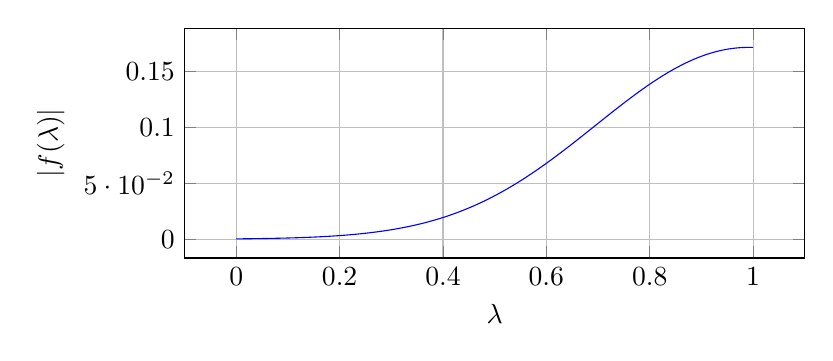
\begin{tikzpicture}
\begin{axis}[width=0.78\textwidth,height=4.5cm,xlabel={$\lambda$},ylabel={$|f(\lambda)|$},grid=major,legend style={font=\small},]
\addplot+[mark=none] coordinates{(0,0.00034216409) (0.0066666667,0.00037145084) (0.013333333,0.00040306783) (0.02,0.00043718292) (0.026666667,0.00047397437) (0.033333333,0.00051363138) (0.04,0.00055635457) (0.046666667,0.0006023565) (0.053333333,0.00065186219) (0.06,0.00070510966) (0.066666667,0.00076235046) (0.073333333,0.00082385019) (0.08,0.00088988909) (0.086666667,0.0009607625) (0.093333333,0.0010367815) (0.1,0.0011182733) (0.10666667,0.0012055819) (0.11333333,0.0012990686) (0.12,0.0013991123) (0.12666667,0.0015061104) (0.13333333,0.0016204786) (0.14,0.0017426521) (0.14666667,0.0018730855) (0.15333333,0.0020122532) (0.16,0.0021606501) (0.16666667,0.0023187916) (0.17333333,0.0024872139) (0.18,0.0026664742) (0.18666667,0.0028571511) (0.19333333,0.0030598444) (0.2,0.0032751753) (0.20666667,0.0035037863) (0.21333333,0.0037463412) (0.22,0.0040035248) (0.22666667,0.0042760428) (0.23333333,0.0045646214) (0.24,0.0048700066) (0.24666667,0.0051929641) (0.25333333,0.0055342786) (0.26,0.0058947527) (0.26666667,0.0062752064) (0.27333333,0.0066764759) (0.28,0.0070994129) (0.28666667,0.0075448831) (0.29333333,0.0080137646) (0.3,0.0085069474) (0.30666667,0.0090253306) (0.31333333,0.0095698218) (0.32,0.010141335) (0.32666667,0.010740787) (0.33333333,0.011369098) (0.34,0.012027189) (0.34666667,0.012715976) (0.35333333,0.013436372) (0.36,0.014189282) (0.36666667,0.0149756) (0.37333333,0.015796209) (0.38,0.016651973) (0.38666667,0.017543739) (0.39333333,0.01847233) (0.4,0.019438546) (0.40666667,0.020443156) (0.41333333,0.021486897) (0.42,0.022570472) (0.42666667,0.023694541) (0.43333333,0.024859726) (0.44,0.026066598) (0.44666667,0.027315681) (0.45333333,0.028607446) (0.46,0.029942303) (0.46666667,0.031320604) (0.47333333,0.032742637) (0.48,0.034208621) (0.48666667,0.035718705) (0.49333333,0.037272961) (0.5,0.038871386) (0.50666667,0.040513896) (0.51333333,0.042200321) (0.52,0.043930408) (0.52666667,0.045703812) (0.53333333,0.047520098) (0.54,0.049378737) (0.54666667,0.051279104) (0.55333333,0.053220477) (0.56,0.055202034) (0.56666667,0.057222855) (0.57333333,0.059281918) (0.58,0.061378097) (0.58666667,0.063510166) (0.59333333,0.065676798) (0.6,0.06787656) (0.60666667,0.070107922) (0.61333333,0.07236925) (0.62,0.074658814) (0.62666667,0.076974782) (0.63333333,0.07931523) (0.64,0.08167814) (0.64666667,0.084061401) (0.65333333,0.086462817) (0.66,0.088880104) (0.66666667,0.091310899) (0.67333333,0.093752762) (0.68,0.09620318) (0.68666667,0.09865957) (0.69333333,0.10111929) (0.7,0.10357963) (0.70666667,0.10603783) (0.71333333,0.1084911) (0.72,0.11093659) (0.72666667,0.1133714) (0.73333333,0.11579264) (0.74,0.11819736) (0.74666667,0.12058262) (0.75333333,0.12294545) (0.76,0.1252829) (0.76666667,0.12759199) (0.77333333,0.12986977) (0.78,0.13211333) (0.78666667,0.13431974) (0.79333333,0.13648612) (0.8,0.13860965) (0.80666667,0.14068752) (0.81333333,0.14271699) (0.82,0.14469537) (0.82666667,0.14662004) (0.83333333,0.14848845) (0.84,0.15029814) (0.84666667,0.15204669) (0.85333333,0.15373182) (0.86,0.1553513) (0.86666667,0.15690304) (0.87333333,0.15838501) (0.88,0.15979532) (0.88666667,0.16113218) (0.89333333,0.16239391) (0.9,0.16357896) (0.90666667,0.16468591) (0.91333333,0.16571343) (0.92,0.16666036) (0.92666667,0.16752564) (0.93333333,0.16830837) (0.94,0.16900774) (0.94666667,0.16962312) (0.95333333,0.17015399) (0.96,0.17059996) (0.96666667,0.1709608) (0.97333333,0.17123638) (0.98,0.17142673) (0.98666667,0.171532) (0.99333333,0.17155248) (1,0.17148857)};
\end{axis}\end{tikzpicture}\end{center}

\end{solution}
\originalsection{第2题：半势阱的Levinson关系（10分）}
\begin{exercise}
半线硬墙加$0<x<a$的$-V_0$势阱, 令$z_0^2=2mV_0a^2/\hbar^2$, $u=ka$, $v=k\prime a=\sqrt{u^2+z_0^2}$. 给定$\tan\delta=(1-(k'/k)\cot(k'a)\tan ka)/(\tan ka+(k'/k)\cot(k'a))$. (a,b)讨论零能及高能极限. (c)写无量纲函数并连续选相移. (d)画$z_0=2,5,9$曲线, 终点分别15、20、30, 检验束缚态数.
\end{exercise}
\begin{solution}
匹配本质为$k\cot(ka+\delta)=k'\cot(k'a)$, 更稳定地写
\[
f(u;z_0)=\frac{u\sin v\cos u-v\cos v\sin u}{u\sin v\sin u+v\cos v\cos u}.
\]
零能$v\to z_0$, 普通非阈值时$\tan\delta\sim u(\tan z_0/z_0-1)\to0$. 题中三例均可取$\delta(0)=0$. 若$z_0=(n+1/2)\pi$恰在零能共振阈值, 此结论需改为半束缚态版本, 不能忽略该例外. 高能$v=u+z_0^2/(2u)+O(u^{-3})$, 匹配与自由波差趋0, 所以$\tan\delta\to0$; 但相移自身可以趋整数倍$\pi$, 不是必须趋0.

计算连续角度$\alpha(u)=\operatorname{unwrap}\arg[v\cos v+\ii u\sin v]$, 令$\delta=\alpha-u-\alpha(0)$, 即避免主值$\arctan$跳跃. 束缚态在$z_0>(n-1/2)\pi$时增加一个, 因此三例$N=1,2,3$. 所选分支应有$\delta(\infty)=-N\pi$, 满足$[\delta(0)-\delta(\infty)]/\pi=N$. 下图终点数值分别$-0.95647\pi,-1.80221\pi,-2.57827\pi$, 距极限仍有$0.04353\pi,0.19779\pi,0.42173\pi$, 大$z_0$需要更高能量才接近极限. 相移加任意固定整数$\pi$不改散射, 两端差不变.
\begin{center}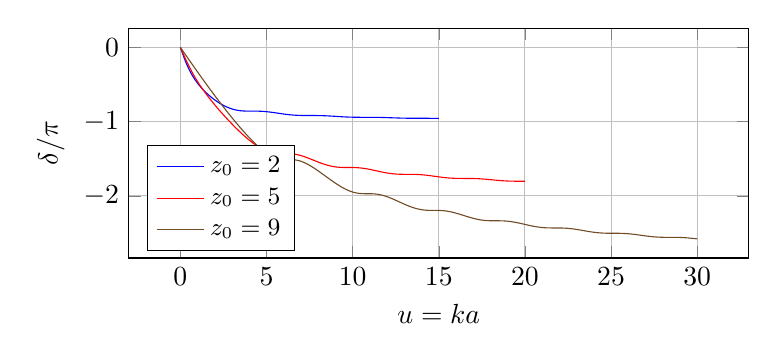
\begin{tikzpicture}
\begin{axis}[width=0.78\textwidth,height=4.5cm,xlabel={$u=ka$},ylabel={$\delta/\pi$},grid=major,legend style={font=\small},legend pos=south west]
\addplot+[mark=none] coordinates{(1e-07,-3.1830989e-08) (0.0500001,-0.033252259) (0.1000001,-0.066201336) (0.1500001,-0.098565366) (0.2000001,-0.13010134) (0.2500001,-0.16061662) (0.3000001,-0.18997346) (0.3500001,-0.21808734) (0.4000001,-0.24492075) (0.4500001,-0.27047465) (0.5000001,-0.29477921) (0.5500001,-0.31788507) (0.6000001,-0.33985597) (0.6500001,-0.36076275) (0.7000001,-0.3806789) (0.75000009,-0.39967743) (0.80000009,-0.41782868) (0.85000009,-0.43519901) (0.90000009,-0.45185009) (0.95000009,-0.46783856) (1.0000001,-0.48321597) (1.0500001,-0.49802896) (1.1000001,-0.51231951) (1.1500001,-0.52612522) (1.2000001,-0.53947969) (1.2500001,-0.55241286) (1.3000001,-0.56495131) (1.3500001,-0.57711862) (1.4000001,-0.58893564) (1.4500001,-0.60042076) (1.5000001,-0.61159015) (1.5500001,-0.622458) (1.6000001,-0.63303667) (1.6500001,-0.64333693) (1.7000001,-0.65336804) (1.7500001,-0.66313798) (1.8000001,-0.67265348) (1.8500001,-0.68192021) (1.9000001,-0.69094283) (1.9500001,-0.69972512) (2.0000001,-0.70827001) (2.0500001,-0.71657971) (2.1000001,-0.72465575) (2.1500001,-0.73249905) (2.2000001,-0.74010998) (2.2500001,-0.74748842) (2.3000001,-0.75463382) (2.3500001,-0.76154524) (2.4000001,-0.76822143) (2.4500001,-0.77466087) (2.5000001,-0.78086181) (2.5500001,-0.78682238) (2.6000001,-0.79254059) (2.6500001,-0.79801446) (2.7000001,-0.80324203) (2.7500001,-0.80822145) (2.8000001,-0.81295108) (2.8500001,-0.81742955) (2.9000001,-0.82165582) (2.9500001,-0.82562931) (3.0000001,-0.82934997) (3.0500001,-0.83281836) (3.1000001,-0.83603574) (3.1500001,-0.83900417) (3.2000001,-0.84172661) (3.2500001,-0.84420695) (3.3000001,-0.84645012) (3.3500001,-0.84846213) (3.4000001,-0.85025015) (3.4500001,-0.85182247) (3.5000001,-0.85318859) (3.5500001,-0.85435916) (3.6000001,-0.85534594) (3.6500001,-0.85616177) (3.7000001,-0.85682047) (3.7500001,-0.85733672) (3.8000001,-0.85772594) (3.8500001,-0.85800415) (3.9000001,-0.85818778) (3.9500001,-0.85829348) (4.0000001,-0.85833794) (4.0500001,-0.85833771) (4.1000001,-0.85830899) (4.1500001,-0.85826743) (4.2000001,-0.85822799) (4.2500001,-0.85820476) (4.3000001,-0.85821085) (4.3500001,-0.85825824) (4.4000001,-0.85835771) (4.4500001,-0.85851879) (4.5000001,-0.85874971) (4.5500001,-0.85905736) (4.6000001,-0.85944733) (4.6500001,-0.85992392) (4.7000001,-0.86049017) (4.7500001,-0.86114795) (4.8000001,-0.86189797) (4.8500001,-0.86273992) (4.9000001,-0.86367249) (4.9500001,-0.8646935) (5.0000001,-0.86579996) (5.0500001,-0.86698816) (5.1000001,-0.86825376) (5.1500001,-0.86959186) (5.2000001,-0.8709971) (5.2500001,-0.8724637) (5.3000001,-0.87398556) (5.3500001,-0.87555631) (5.4000001,-0.87716937) (5.4500001,-0.87881801) (5.5000001,-0.88049541) (5.5500001,-0.88219469) (5.6000001,-0.88390896) (5.6500001,-0.88563138) (5.7000001,-0.88735518) (5.7500001,-0.8890737) (5.8000001,-0.89078041) (5.8500001,-0.89246899) (5.9000001,-0.8941333) (5.9500001,-0.89576746) (6.0000001,-0.89736585) (6.0500001,-0.89892314) (6.1000001,-0.90043433) (6.1500001,-0.90189476) (6.2000001,-0.90330016) (6.2500001,-0.90464666) (6.3000001,-0.90593079) (6.3500001,-0.90714954) (6.4000001,-0.90830037) (6.4500001,-0.90938121) (6.5000001,-0.9103905) (6.5500001,-0.91132718) (6.6000001,-0.91219074) (6.6500001,-0.91298116) (6.7000001,-0.91369899) (6.7500001,-0.91434529) (6.8000001,-0.91492166) (6.8500001,-0.91543019) (6.9000001,-0.91587349) (6.9500001,-0.91625463) (7.0000001,-0.91657714) (7.0500001,-0.91684494) (7.1000001,-0.91706236) (7.1500001,-0.91723403) (7.2000001,-0.91736488) (7.2500001,-0.91746007) (7.3000001,-0.91752494) (7.3500001,-0.91756496) (7.4000001,-0.91758564) (7.4500001,-0.91759253) (7.5000001,-0.91759109) (7.55,-0.91758671) (7.6,-0.91758459) (7.65,-0.91758973) (7.7,-0.91760685) (7.75,-0.91764039) (7.8,-0.91769443) (7.85,-0.91777269) (7.9,-0.91787849) (7.95,-0.91801471) (8,-0.91818381) (8.05,-0.9183878) (8.1,-0.91862825) (8.15,-0.91890628) (8.2,-0.91922255) (8.25,-0.9195773) (8.3,-0.91997038) (8.35,-0.9204012) (8.4,-0.92086881) (8.45,-0.92137191) (8.5,-0.92190887) (8.55,-0.92247776) (8.6,-0.92307635) (8.65,-0.92370222) (8.7,-0.92435267) (8.75,-0.92502487) (8.8,-0.9257158) (8.85,-0.92642233) (8.9,-0.92714124) (8.95,-0.92786924) (9,-0.92860298) (9.05,-0.92933913) (9.1,-0.93007437) (9.15,-0.93080542) (9.2,-0.93152906) (9.25,-0.93224219) (9.3,-0.9329418) (9.35,-0.93362502) (9.4,-0.93428917) (9.45,-0.93493172) (9.5,-0.93555036) (9.55,-0.93614296) (9.6,-0.93670767) (9.65,-0.93724285) (9.7,-0.93774712) (9.75,-0.93821939) (9.8,-0.93865882) (9.85,-0.93906486) (9.9,-0.93943725) (9.95,-0.939776) (10,-0.94008141) (10.05,-0.94035406) (10.1,-0.94059482) (10.15,-0.94080478) (10.2,-0.94098532) (10.25,-0.94113804) (10.3,-0.94126476) (10.35,-0.9413675) (10.4,-0.94144847) (10.45,-0.94151001) (10.5,-0.94155462) (10.55,-0.94158487) (10.6,-0.94160344) (10.65,-0.94161303) (10.7,-0.94161639) (10.75,-0.94161623) (10.8,-0.94161524) (10.85,-0.94161606) (10.9,-0.94162121) (10.95,-0.94163313) (11,-0.94165411) (11.05,-0.94168627) (11.1,-0.94173158) (11.15,-0.94179181) (11.2,-0.94186852) (11.25,-0.94196307) (11.3,-0.94207658) (11.35,-0.94220995) (11.4,-0.94236384) (11.45,-0.9425387) (11.5,-0.94273473) (11.55,-0.9429519) (11.6,-0.94318997) (11.65,-0.94344848) (11.7,-0.94372677) (11.75,-0.94402399) (11.8,-0.94433912) (11.85,-0.94467094) (11.9,-0.94501812) (11.95,-0.94537918) (12,-0.94575252) (12.05,-0.94613644) (12.1,-0.94652916) (12.15,-0.94692882) (12.2,-0.94733355) (12.25,-0.94774141) (12.3,-0.94815046) (12.35,-0.94855878) (12.4,-0.94896445) (12.45,-0.9493656) (12.5,-0.94976042) (12.55,-0.95014716) (12.6,-0.95052415) (12.65,-0.95088984) (12.7,-0.95124278) (12.75,-0.95158163) (12.8,-0.9519052) (12.85,-0.95221244) (12.9,-0.95250245) (12.95,-0.95277449) (13,-0.95302799) (13.05,-0.95326254) (13.1,-0.9534779) (13.15,-0.95367401) (13.2,-0.95385098) (13.25,-0.9540091) (13.3,-0.95414879) (13.35,-0.95427066) (13.4,-0.95437549) (13.45,-0.95446415) (13.5,-0.9545377) (13.55,-0.9545973) (13.6,-0.95464421) (13.65,-0.9546798) (13.7,-0.95470554) (13.75,-0.95472294) (13.8,-0.95473357) (13.85,-0.95473903) (13.9,-0.95474097) (13.95,-0.954741) (14,-0.95474073) (14.05,-0.95474176) (14.1,-0.95474562) (14.15,-0.95475378) (14.2,-0.95476765) (14.25,-0.95478853) (14.3,-0.95481765) (14.35,-0.9548561) (14.4,-0.95490486) (14.45,-0.9549648) (14.5,-0.95503664) (14.55,-0.95512095) (14.6,-0.95521819) (14.65,-0.95532865) (14.7,-0.95545249) (14.75,-0.95558972) (14.8,-0.95574021) (14.85,-0.95590372) (14.9,-0.95607983) (14.95,-0.95626805) (15,-0.95646773)};
\addlegendentry{$z_0=2$}
\addplot+[mark=none] coordinates{(1e-07,-3.1830989e-08) (0.066666766,-0.035533708) (0.13333343,-0.070863755) (0.2000001,-0.10579805) (0.26666677,-0.14016595) (0.33333343,-0.17382546) (0.4000001,-0.20666719) (0.46666676,-0.23861497) (0.53333343,-0.26962395) (0.6000001,-0.29967677) (0.66666676,-0.32877877) (0.73333343,-0.35695299) (0.8000001,-0.38423544) (0.86666676,-0.41067083) (0.93333343,-0.43630919) (1.0000001,-0.46120304) (1.0666668,-0.48540535) (1.1333334,-0.50896799) (1.2000001,-0.53194073) (1.2666668,-0.55437055) (1.3333334,-0.57630125) (1.4000001,-0.59777325) (1.4666668,-0.61882357) (1.5333334,-0.63948589) (1.6000001,-0.65979067) (1.6666668,-0.67976533) (1.7333334,-0.69943443) (1.8000001,-0.71881987) (1.8666668,-0.73794112) (1.9333334,-0.75681539) (2.0000001,-0.7754578) (2.0666668,-0.7938816) (2.1333334,-0.81209829) (2.2000001,-0.83011778) (2.2666668,-0.84794854) (2.3333334,-0.8655977) (2.4000001,-0.88307113) (2.4666668,-0.90037361) (2.5333334,-0.91750886) (2.6000001,-0.93447959) (2.6666668,-0.95128764) (2.7333334,-0.96793395) (2.8000001,-0.98441869) (2.8666668,-1.0007412) (2.9333334,-1.0169001) (3.0000001,-1.0328934) (3.0666668,-1.0487181) (3.1333334,-1.0643708) (3.2000001,-1.0798474) (3.2666668,-1.0951428) (3.3333334,-1.1102516) (3.4000001,-1.1251675) (3.4666667,-1.1398834) (3.5333334,-1.1543917) (3.6000001,-1.1686838) (3.6666667,-1.1827505) (3.7333334,-1.1965817) (3.8000001,-1.2101665) (3.8666667,-1.2234931) (3.9333334,-1.2365489) (4.0000001,-1.2493202) (4.0666667,-1.2617925) (4.1333334,-1.2739505) (4.2000001,-1.2857775) (4.2666667,-1.2972564) (4.3333334,-1.3083687) (4.4000001,-1.3190953) (4.4666667,-1.3294164) (4.5333334,-1.3393113) (4.6000001,-1.3487589) (4.6666667,-1.3577381) (4.7333334,-1.3662275) (4.8000001,-1.3742064) (4.8666667,-1.381655) (4.9333334,-1.3885548) (5.0000001,-1.39489) (5.0666667,-1.4006472) (5.1333334,-1.4058175) (5.2000001,-1.4103966) (5.2666667,-1.4143863) (5.3333334,-1.4177951) (5.4000001,-1.4206398) (5.4666667,-1.4229458) (5.5333334,-1.4247477) (5.6000001,-1.4260895) (5.6666667,-1.4270245) (5.7333334,-1.4276145) (5.8000001,-1.4279285) (5.8666667,-1.4280407) (5.9333334,-1.4280288) (6.0000001,-1.4279715) (6.0666667,-1.4279457) (6.1333334,-1.4280245) (6.2000001,-1.4282751) (6.2666667,-1.4287568) (6.3333334,-1.4295203) (6.4000001,-1.4306063) (6.4666667,-1.432046) (6.5333334,-1.4338611) (6.6000001,-1.4360641) (6.6666667,-1.4386595) (6.7333334,-1.4416445) (6.8000001,-1.4450103) (6.8666667,-1.4487425) (6.9333334,-1.452823) (7.0000001,-1.4572301) (7.0666667,-1.4619395) (7.1333334,-1.4669253) (7.2000001,-1.4721599) (7.2666667,-1.4776152) (7.3333334,-1.4832622) (7.4000001,-1.4890722) (7.4666667,-1.4950159) (7.5333334,-1.5010647) (7.6000001,-1.5071898) (7.6666667,-1.5133631) (7.7333334,-1.5195568) (7.8000001,-1.5257435) (7.8666667,-1.5318962) (7.9333334,-1.5379886) (8.0000001,-1.5439949) (8.0666667,-1.5498897) (8.1333334,-1.5556483) (8.2000001,-1.5612469) (8.2666667,-1.5666623) (8.3333334,-1.5718723) (8.4000001,-1.5768557) (8.4666667,-1.5815926) (8.5333334,-1.5860646) (8.6000001,-1.5902552) (8.6666667,-1.5941499) (8.7333334,-1.5977364) (8.8000001,-1.6010053) (8.8666667,-1.6039503) (8.9333334,-1.6065688) (9.0000001,-1.6088616) (9.0666667,-1.610834) (9.1333334,-1.6124957) (9.2000001,-1.6138607) (9.2666667,-1.614948) (9.3333334,-1.6157807) (9.4000001,-1.6163866) (9.4666667,-1.616797) (9.5333334,-1.6170468) (9.6000001,-1.6171732) (9.6666667,-1.6172153) (9.7333334,-1.6172129) (9.8000001,-1.6172057) (9.8666667,-1.6172322) (9.9333334,-1.6173288) (10,-1.6175291) (10.066667,-1.6178632) (10.133333,-1.6183571) (10.2,-1.6190325) (10.266667,-1.6199063) (10.333333,-1.620991) (10.4,-1.6222943) (10.466667,-1.6238199) (10.533333,-1.6255672) (10.6,-1.6275321) (10.666667,-1.6297071) (10.733333,-1.6320817) (10.8,-1.6346431) (10.866667,-1.6373763) (10.933333,-1.6402644) (11,-1.6432892) (11.066667,-1.6464314) (11.133333,-1.6496707) (11.2,-1.6529864) (11.266667,-1.6563572) (11.333333,-1.6597618) (11.4,-1.6631786) (11.466667,-1.6665865) (11.533333,-1.6699645) (11.6,-1.6732921) (11.666667,-1.6765495) (11.733333,-1.6797175) (11.8,-1.6827782) (11.866667,-1.6857143) (11.933333,-1.6885102) (12,-1.6911516) (12.066667,-1.6936258) (12.133333,-1.6959221) (12.2,-1.6980317) (12.266667,-1.6999481) (12.333333,-1.7016674) (12.4,-1.7031881) (12.466667,-1.7045115) (12.533333,-1.7056417) (12.6,-1.7065858) (12.666667,-1.7073536) (12.733333,-1.7079578) (12.8,-1.7084138) (12.866667,-1.7087392) (12.933333,-1.708954) (13,-1.7090796) (13.066667,-1.709139) (13.133333,-1.7091557) (13.2,-1.7091538) (13.266667,-1.709157) (13.333333,-1.7091883) (13.4,-1.7092696) (13.466667,-1.7094209) (13.533333,-1.7096604) (13.6,-1.710004) (13.666667,-1.7104648) (13.733333,-1.7110536) (13.8,-1.7117781) (13.866667,-1.7126433) (13.933333,-1.7136517) (14,-1.714803) (14.066667,-1.7160946) (14.133333,-1.7175215) (14.2,-1.7190768) (14.266667,-1.7207518) (14.333333,-1.7225361) (14.4,-1.7244179) (14.466667,-1.7263844) (14.533333,-1.7284218) (14.6,-1.7305155) (14.666667,-1.7326506) (14.733333,-1.7348115) (14.8,-1.7369829) (14.866667,-1.7391491) (14.933333,-1.7412949) (15,-1.7434054) (15.066667,-1.745466) (15.133333,-1.7474631) (15.2,-1.7493837) (15.266667,-1.7512159) (15.333333,-1.752949) (15.4,-1.7545735) (15.466667,-1.7560812) (15.533333,-1.7574659) (15.6,-1.7587227) (15.666667,-1.7598487) (15.733333,-1.7608429) (15.8,-1.7617061) (15.866667,-1.7624413) (15.933333,-1.7630534) (16,-1.7635492) (16.066667,-1.7639375) (16.133333,-1.7642288) (16.2,-1.764435) (16.266667,-1.7645696) (16.333333,-1.764647) (16.4,-1.7646824) (16.466667,-1.7646917) (16.533333,-1.7646909) (16.6,-1.7646958) (16.666667,-1.7647217) (16.733333,-1.7647832) (16.8,-1.7648939) (16.866667,-1.765066) (16.933333,-1.7653104) (17,-1.7656362) (17.066667,-1.7660507) (17.133333,-1.7665594) (17.2,-1.767166) (17.266667,-1.7678723) (17.333333,-1.7686783) (17.4,-1.7695822) (17.466667,-1.7705808) (17.533333,-1.771669) (17.6,-1.7728407) (17.666667,-1.7740885) (17.733333,-1.7754038) (17.8,-1.7767772) (17.866667,-1.7781986) (17.933333,-1.7796573) (18,-1.781142) (18.066667,-1.7826415) (18.133333,-1.7841441) (18.2,-1.7856384) (18.266667,-1.7871132) (18.333333,-1.7885574) (18.4,-1.7899607) (18.466667,-1.7913132) (18.533333,-1.7926056) (18.6,-1.7938299) (18.666667,-1.7949787) (18.733333,-1.7960459) (18.8,-1.7970265) (18.866667,-1.7979168) (18.933333,-1.7987146) (19,-1.7994189) (19.066667,-1.8000303) (19.133333,-1.8005509) (19.2,-1.800984) (19.266667,-1.8013347) (19.333333,-1.8016091) (19.4,-1.8018147) (19.466667,-1.8019601) (19.533333,-1.8020547) (19.6,-1.802109) (19.666667,-1.8021338) (19.733333,-1.8021404) (19.8,-1.8021401) (19.866667,-1.8021443) (19.933333,-1.802164) (20,-1.8022096)};
\addlegendentry{$z_0=5$}
\addplot+[mark=none] coordinates{(1e-07,-3.1830989e-08) (0.1000001,-0.033428282) (0.2000001,-0.066841683) (0.3000001,-0.10022549) (0.4000001,-0.13356518) (0.5000001,-0.16684651) (0.6000001,-0.20005564) (0.7000001,-0.2331792) (0.8000001,-0.26620435) (0.9000001,-0.29911884) (1.0000001,-0.33191104) (1.1000001,-0.36456993) (1.2000001,-0.39708517) (1.3000001,-0.42944703) (1.4000001,-0.46164639) (1.5000001,-0.49367471) (1.6000001,-0.52552395) (1.7000001,-0.55718654) (1.8000001,-0.5886553) (1.9000001,-0.61992335) (2.0000001,-0.65098403) (2.1000001,-0.68183081) (2.2000001,-0.71245721) (2.3000001,-0.74285664) (2.4000001,-0.77302235) (2.5000001,-0.80294729) (2.6000001,-0.83262396) (2.7000001,-0.86204433) (2.8000001,-0.89119968) (2.9000001,-0.92008046) (3.0000001,-0.9486761) (3.1000001,-0.97697489) (3.2000001,-1.0049638) (3.3000001,-1.0326281) (3.4000001,-1.0599514) (3.5000001,-1.0869153) (3.6000001,-1.113499) (3.7000001,-1.139679) (3.8000001,-1.1654289) (3.9000001,-1.1907188) (4.0000001,-1.2155151) (4.1000001,-1.2397795) (4.2000001,-1.2634692) (4.3000001,-1.2865357) (4.4000001,-1.3089244) (4.5000001,-1.3305739) (4.6000001,-1.3514156) (4.7000001,-1.3713728) (4.8000001,-1.3903611) (4.9000001,-1.4082875) (5.0000001,-1.4250522) (5.1000001,-1.4405491) (5.2000001,-1.4546694) (5.3000001,-1.4673064) (5.4000001,-1.4783621) (5.5000001,-1.4877576) (5.6000001,-1.4954461) (5.7000001,-1.5014282) (5.8000001,-1.5057685) (5.9000001,-1.5086099) (6.0000001,-1.5101818) (6.1000001,-1.5107972) (6.2000001,-1.5108373) (6.3000001,-1.5107218) (6.4000001,-1.5108718) (6.5000001,-1.5116725) (6.6000001,-1.5134425) (6.7000001,-1.5164168) (6.8000001,-1.5207427) (6.9000001,-1.5264873) (7.0000001,-1.5336513) (7.1000001,-1.5421854) (7.2000001,-1.5520058) (7.3000001,-1.5630074) (7.4000001,-1.5750742) (7.5000001,-1.5880866) (7.6000001,-1.601926) (7.7000001,-1.6164779) (7.8000001,-1.6316338) (7.9000001,-1.6472912) (8.0000001,-1.6633538) (8.1000001,-1.6797315) (8.2000001,-1.6963388) (8.3000001,-1.713095) (8.4000001,-1.7299226) (8.5000001,-1.7467468) (8.6000001,-1.7634943) (8.7000001,-1.7800928) (8.8000001,-1.7964702) (8.9000001,-1.8125535) (9.0000001,-1.8282686) (9.1000001,-1.8435394) (9.2000001,-1.8582879) (9.3000001,-1.8724335) (9.4000001,-1.8858936) (9.5000001,-1.898584) (9.6000001,-1.9104201) (9.7000001,-1.9213187) (9.8000001,-1.9312008) (9.9000001,-1.9399957) (10,-1.9476459) (10.1,-1.9541135) (10.2,-1.9593874) (10.3,-1.9634909) (10.4,-1.9664888) (10.5,-1.9684915) (10.6,-1.9696572) (10.7,-1.9701871) (10.8,-1.9703165) (10.9,-1.9703003) (11,-1.9703954) (11.1,-1.9708425) (11.2,-1.9718512) (11.3,-1.9735887) (11.4,-1.9761744) (11.5,-1.9796802) (11.6,-1.9841343) (11.7,-1.9895275) (11.8,-1.995821) (11.9,-2.0029533) (12,-2.0108472) (12.1,-2.019415) (12.2,-2.0285625) (12.3,-2.0381926) (12.4,-2.0482066) (12.5,-2.0585063) (12.6,-2.0689942) (12.7,-2.0795744) (12.8,-2.0901522) (12.9,-2.1006345) (13,-2.1109297) (13.1,-2.1209477) (13.2,-2.1306) (13.3,-2.1398008) (13.4,-2.1484671) (13.5,-2.1565205) (13.6,-2.1638892) (13.7,-2.1705101) (13.8,-2.1763323) (13.9,-2.1813208) (14,-2.1854602) (14.1,-2.1887594) (14.2,-2.1912545) (14.3,-2.1930119) (14.4,-2.1941284) (14.5,-2.1947295) (14.6,-2.1949646) (14.7,-2.1949994) (14.8,-2.1950066) (14.9,-2.1951557) (15,-2.1956027) (15.1,-2.1964819) (15.2,-2.1979002) (15.3,-2.1999342) (15.4,-2.2026295) (15.5,-2.2060029) (15.6,-2.2100454) (15.7,-2.2147268) (15.8,-2.2199989) (15.9,-2.2258006) (16,-2.2320608) (16.1,-2.2387011) (16.2,-2.245639) (16.3,-2.2527888) (16.4,-2.2600638) (16.5,-2.2673769) (16.6,-2.2746417) (16.7,-2.2817733) (16.8,-2.2886892) (16.9,-2.29531) (17,-2.3015611) (17.1,-2.3073733) (17.2,-2.3126853) (17.3,-2.3174452) (17.4,-2.3216132) (17.5,-2.3251641) (17.6,-2.3280896) (17.7,-2.3304009) (17.8,-2.3321304) (17.9,-2.3333323) (18,-2.3340821) (18.1,-2.3344746) (18.2,-2.3346197) (18.3,-2.3346376) (18.4,-2.3346518) (18.5,-2.3347831) (18.6,-2.3351429) (18.7,-2.3358274) (18.8,-2.3369145) (18.9,-2.3384607) (19,-2.3405006) (19.1,-2.343048) (19.2,-2.3460971) (19.3,-2.3496251) (19.4,-2.3535951) (19.5,-2.3579582) (19.6,-2.3626568) (19.7,-2.3676263) (19.8,-2.3727974) (19.9,-2.3780979) (20,-2.383454) (20.1,-2.3887915) (20.2,-2.3940376) (20.3,-2.3991216) (20.4,-2.4039761) (20.5,-2.4085389) (20.6,-2.4127537) (20.7,-2.4165725) (20.8,-2.4199569) (20.9,-2.4228799) (21,-2.4253281) (21.1,-2.4273027) (21.2,-2.4288214) (21.3,-2.4299182) (21.4,-2.4306435) (21.5,-2.4310627) (21.6,-2.4312538) (21.7,-2.4313041) (21.8,-2.4313055) (21.9,-2.4313506) (22,-2.4315274) (22.1,-2.4319153) (22.2,-2.4325818) (22.3,-2.4335797) (22.4,-2.4349457) (22.5,-2.4367005) (22.6,-2.4388486) (22.7,-2.4413802) (22.8,-2.4442725) (22.9,-2.4474914) (23,-2.4509941) (23.1,-2.4547303) (23.2,-2.4586445) (23.3,-2.4626774) (23.4,-2.4667678) (23.5,-2.4708536) (23.6,-2.4748733) (23.7,-2.4787674) (23.8,-2.4824796) (23.9,-2.4859583) (24,-2.4891578) (24.1,-2.49204) (24.2,-2.4945754) (24.3,-2.4967452) (24.4,-2.4985419) (24.5,-2.4999705) (24.6,-2.5010492) (24.7,-2.5018092) (24.8,-2.5022942) (24.9,-2.5025588) (25,-2.5026664) (25.1,-2.5026864) (25.2,-2.502691) (25.3,-2.5027514) (25.4,-2.5029348) (25.5,-2.5033013) (25.6,-2.503901) (25.7,-2.5047726) (25.8,-2.5059425) (25.9,-2.507424) (26,-2.5092182) (26.1,-2.5113145) (26.2,-2.5136922) (26.3,-2.5163213) (26.4,-2.5191646) (26.5,-2.522179) (26.6,-2.525317) (26.7,-2.5285284) (26.8,-2.5317613) (26.9,-2.5349638) (27,-2.5380851) (27.1,-2.5410766) (27.2,-2.5438938) (27.3,-2.5464969) (27.4,-2.5488523) (27.5,-2.5509339) (27.6,-2.5527243) (27.7,-2.5542154) (27.8,-2.5554095) (27.9,-2.5563196) (28,-2.5569692) (28.1,-2.5573919) (28.2,-2.5576303) (28.3,-2.557734) (28.4,-2.5577581) (28.5,-2.55776) (28.6,-2.5577972) (28.7,-2.5579244) (28.8,-2.558191) (28.9,-2.5586394) (29,-2.5593032) (29.1,-2.5602058) (29.2,-2.5613609) (29.3,-2.5627714) (29.4,-2.5644309) (29.5,-2.5663239) (29.6,-2.5684271) (29.7,-2.5707105) (29.8,-2.5731389) (29.9,-2.5756728) (30,-2.57827)};
\addlegendentry{$z_0=9$}
\end{axis}\end{tikzpicture}\end{center}

\end{solution}
\originalsection{第3题：台阶与硬墙（10分）}
\begin{exercise}
半线$0<x<a$势$V_0>0$, $x>a$势0, 左端硬墙. (a)对$E>V_0$求$\cot\delta$. (b)对$E<V_0$求同式. (c)画$z_0=5$时从零能到高能的相移.
\end{exercise}
\begin{solution}
外部取$\sin(kx+\delta)$, 内部高能取$A\sin(qx)$, $q=\sqrt{2m(E-V_0)}/\hbar$. 令$C=(q/k)\cot qa$, 匹配$\cot(u+\delta)=C$, 解得$\cot\delta=(1+C\cot u)/(\cot u-C)$. 低能内部取$A\sinh\kappa x$, 因而同式只需$C=(\kappa/k)\coth\kappa a$, $\kappa=\sqrt{2m(V_0-E)}/\hbar$. 在$E=V_0$内解为线性, 连续极限$C=1/u$. 绘图先取$u+\delta$的连续辐角再减$u$, 不把不同主值支路拼接. $\delta(0)=0$, 中间为负（排斥使外波等效向外平移）, $u\to\infty$时从负侧趋0, 无束缚态. 下图画至35; 无限区间的末段由$\delta\sim-z_0^2/(2u)$描述.
\begin{center}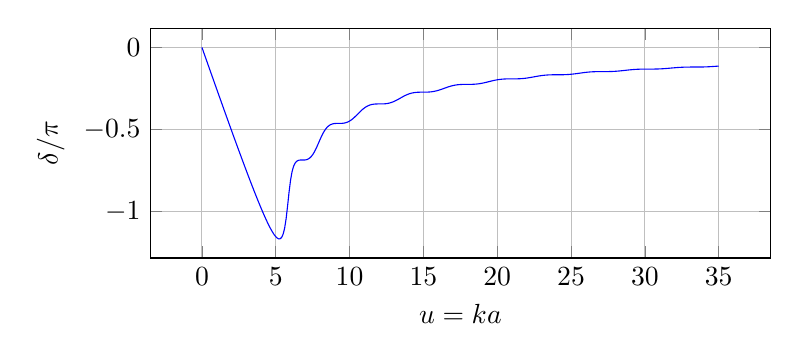
\begin{tikzpicture}
\begin{axis}[width=0.78\textwidth,height=4.5cm,xlabel={$u=ka$},ylabel={$\delta/\pi$},grid=major,legend style={font=\small},]
\addplot+[mark=none] coordinates{(1e-07,-2.5465369e-08) (0.1000001,-0.025464971) (0.2000001,-0.050927374) (0.3000001,-0.076384683) (0.4000001,-0.10183433) (0.5000001,-0.12727371) (0.6000001,-0.1527002) (0.7000001,-0.17811111) (0.8000001,-0.2035037) (0.9000001,-0.22887517) (1.0000001,-0.25422263) (1.1000001,-0.27954308) (1.2000001,-0.30483346) (1.3000001,-0.33009054) (1.4000001,-0.35531098) (1.5000001,-0.38049128) (1.6000001,-0.40562775) (1.7000001,-0.43071652) (1.8000001,-0.45575349) (1.9000001,-0.4807343) (2.0000001,-0.50565433) (2.1000001,-0.53050863) (2.2000001,-0.55529188) (2.3000001,-0.57999837) (2.4000001,-0.60462193) (2.5000001,-0.62915585) (2.6000001,-0.65359284) (2.7000001,-0.67792493) (2.8000001,-0.70214334) (2.9000001,-0.72623841) (3.0000001,-0.75019942) (3.1000001,-0.77401443) (3.2000001,-0.79767007) (3.3000001,-0.82115129) (3.4000001,-0.84444103) (3.5000001,-0.86751986) (3.6000001,-0.89036548) (3.7000001,-0.91295211) (3.8000001,-0.93524972) (3.9000001,-0.95722306) (4.0000001,-0.9788303) (4.1000001,-1.0000214) (4.2000001,-1.0207358) (4.3000001,-1.0408992) (4.4000001,-1.0604196) (4.5000001,-1.0791811) (4.6000001,-1.0970353) (4.7000001,-1.1137891) (4.8000001,-1.129186) (4.9000001,-1.1428783) (5.0000001,-1.1543824) (5.1000001,-1.1630092) (5.2000001,-1.1677497) (5.3000001,-1.1670883) (5.4000001,-1.1587085) (5.5000001,-1.1390941) (5.6000001,-1.1033069) (5.7000001,-1.0462851) (5.8000001,-0.96855434) (5.9000001,-0.88372452) (6.0000001,-0.81130121) (6.1000001,-0.75989541) (6.2000001,-0.72700145) (6.3000001,-0.70718603) (6.4000001,-0.69592257) (6.5000001,-0.69007325) (6.6000001,-0.68752774) (6.7000001,-0.68682988) (6.8000001,-0.68692258) (6.9000001,-0.6869888) (7.0000001,-0.68635531) (7.1000001,-0.68443691) (7.2000001,-0.68070953) (7.3000001,-0.67470843) (7.4000001,-0.66605168) (7.5000001,-0.65449022) (7.6000001,-0.63998048) (7.7000001,-0.62276289) (7.8000001,-0.60341167) (7.9000001,-0.58281278) (8.0000001,-0.5620456) (8.1000001,-0.54219354) (8.2000001,-0.52415439) (8.3000001,-0.5085219) (8.4000001,-0.49556428) (8.5000001,-0.48527636) (8.6000001,-0.47746246) (8.7000001,-0.47181594) (8.8000001,-0.46797973) (8.9000001,-0.46558552) (9.0000001,-0.46427582) (9.1000001,-0.46371443) (9.2000001,-0.46359013) (9.3000001,-0.46361694) (9.4000001,-0.4635332) (9.5000001,-0.46310103) (9.6000001,-0.46210709) (9.7000001,-0.46036523) (9.8000001,-0.45772139) (9.9000001,-0.45406089) (10,-0.44931732) (10.1,-0.44348207) (10.2,-0.43661245) (10.3,-0.42883575) (10.4,-0.42034653) (10.5,-0.41139544) (10.6,-0.40226953) (10.7,-0.39326645) (10.8,-0.3846672) (10.9,-0.37671212) (11,-0.36958422) (11.1,-0.36340154) (11.2,-0.35821766) (11.3,-0.35402852) (11.4,-0.3507826) (11.5,-0.34839209) (11.6,-0.34674356) (11.7,-0.34570703) (11.8,-0.34514332) (11.9,-0.34490972) (12,-0.34486426) (12.1,-0.34486916) (12.2,-0.34479357) (12.3,-0.34451618) (12.4,-0.34392786) (12.5,-0.34293441) (12.6,-0.34145969) (12.7,-0.33944883) (12.8,-0.33687145) (12.9,-0.33372444) (13,-0.33003377) (13.1,-0.32585491) (13.2,-0.32127111) (13.3,-0.31638952) (13.4,-0.3113349) (13.5,-0.30624166) (13.6,-0.30124482) (13.7,-0.29647102) (13.8,-0.29203076) (13.9,-0.28801241) (14,-0.28447865) (14.1,-0.28146525) (14.2,-0.27898189) (14.3,-0.27701451) (14.4,-0.27552862) (14.5,-0.27447308) (14.6,-0.27378391) (14.7,-0.27338794) (14.8,-0.27320614) (14.9,-0.2731566) (15,-0.27315716) (15.1,-0.27312787) (15.2,-0.27299318) (15.3,-0.27268408) (15.4,-0.2721402) (15.5,-0.27131176) (15.6,-0.27016155) (15.7,-0.26866654) (15.8,-0.26681933) (15.9,-0.26462894) (16,-0.26212095) (16.1,-0.25933674) (16.2,-0.25633176) (16.3,-0.25317281) (16.4,-0.24993445) (16.5,-0.2466948) (16.6,-0.24353112) (16.7,-0.24051551) (16.8,-0.23771113) (16.9,-0.23516926) (17,-0.23292731) (17.1,-0.23100784) (17.2,-0.22941859) (17.3,-0.22815324) (17.4,-0.22719277) (17.5,-0.22650726) (17.6,-0.22605785) (17.7,-0.22579881) (17.8,-0.22567961) (17.9,-0.22564694) (18,-0.22564652) (18.1,-0.22562501) (18.2,-0.22553162) (18.3,-0.2253198) (18.4,-0.22494874) (18.5,-0.2243848) (18.6,-0.22360278) (18.7,-0.22258697) (18.8,-0.22133197) (18.9,-0.21984312) (19,-0.21813641) (19.1,-0.216238) (19.2,-0.21418311) (19.3,-0.21201435) (19.4,-0.20977967) (19.5,-0.20752988) (19.6,-0.20531604) (19.7,-0.2031869) (19.8,-0.20118643) (19.9,-0.19935189) (20,-0.19771228) (20.1,-0.19628734) (20.2,-0.19508718) (20.3,-0.19411235) (20.4,-0.19335439) (20.5,-0.19279667) (20.6,-0.19241556) (20.7,-0.19218165) (20.8,-0.1920612) (20.9,-0.19201747) (21,-0.1920122) (21.1,-0.19200693) (21.2,-0.19196433) (21.3,-0.19184953) (21.4,-0.19163126) (21.5,-0.19128296) (21.6,-0.19078378) (21.7,-0.19011939) (21.8,-0.18928258) (21.9,-0.18827365) (22,-0.18710049) (22.1,-0.18577829) (22.2,-0.18432895) (22.3,-0.18278013) (22.4,-0.18116395) (22.5,-0.17951544) (22.6,-0.17787091) (22.7,-0.17626614) (22.8,-0.17473472) (22.9,-0.17330649) (23,-0.1720063) (23.1,-0.17085301) (23.2,-0.16985893) (23.3,-0.16902953) (23.4,-0.16836351) (23.5,-0.16785321) (23.6,-0.16748514) (23.7,-0.16724082) (23.8,-0.16709767) (23.9,-0.16702999) (24,-0.16701004) (24.1,-0.1670091) (24.2,-0.1669985) (24.3,-0.16695064) (24.4,-0.16684001) (24.5,-0.16664406) (24.6,-0.16634404) (24.7,-0.16592569) (24.8,-0.16537983) (24.9,-0.16470272) (25,-0.16389627) (25.1,-0.16296797) (25.2,-0.16193066) (25.3,-0.16080191) (25.4,-0.15960332) (25.5,-0.1583595) (25.6,-0.15709697) (25.7,-0.15584287) (25.8,-0.15462377) (25.9,-0.15346443) (26,-0.15238674) (26.1,-0.15140878) (26.2,-0.15054419) (26.3,-0.14980167) (26.4,-0.14918481) (26.5,-0.14869215) (26.6,-0.14831737) (26.7,-0.14804978) (26.8,-0.14787485) (26.9,-0.14777493) (27,-0.14772997) (27.1,-0.14771838) (27.2,-0.14771783) (27.3,-0.14770609) (27.4,-0.14766184) (27.5,-0.14756546) (27.6,-0.14739974) (27.7,-0.1471505) (27.8,-0.14680715) (27.9,-0.1463631) (28,-0.14581601) (28.1,-0.14516796) (28.2,-0.1444253) (28.3,-0.14359845) (28.4,-0.14270146) (28.5,-0.14175136) (28.6,-0.14076742) (28.7,-0.13977032) (28.8,-0.13878117) (28.9,-0.13782055) (29,-0.13690769) (29.1,-0.13605956) (29.2,-0.1352902) (29.3,-0.13461024) (29.4,-0.13402648) (29.5,-0.13354175) (29.6,-0.1331549) (29.7,-0.13286099) (29.8,-0.13265158) (29.9,-0.13251519) (30,-0.13243779) (30.1,-0.13240344) (30.2,-0.13239493) (30.3,-0.1323944) (30.4,-0.13238409) (30.5,-0.13234695) (30.6,-0.13226728) (30.7,-0.13213134) (30.8,-0.1319278) (30.9,-0.13164826) (31,-0.1312875) (31.1,-0.13084373) (31.2,-0.13031865) (31.3,-0.1297174) (31.4,-0.12904835) (31.5,-0.12832272) (31.6,-0.12755413) (31.7,-0.12675799) (31.8,-0.12595081) (31.9,-0.12514949) (32,-0.12437055) (32.1,-0.12362946) (32.2,-0.12293995) (32.3,-0.12231347) (32.4,-0.12175877) (32.5,-0.12128154) (32.6,-0.12088433) (32.7,-0.12056646) (32.8,-0.12032419) (32.9,-0.12015088) (33,-0.12003739) (33.1,-0.11997247) (33.2,-0.11994323) (33.3,-0.11993566) (33.4,-0.11993522) (33.5,-0.11992733) (33.6,-0.11989799) (33.7,-0.11983425) (33.8,-0.11972474) (33.9,-0.11956005) (34,-0.11933313) (34.1,-0.11903953) (34.2,-0.11867762) (34.3,-0.11824861) (34.4,-0.11775652) (34.5,-0.11720801) (34.6,-0.11661211) (34.7,-0.11597984) (34.8,-0.11532369) (34.9,-0.11465712) (35,-0.11399398)};
\end{axis}\end{tikzpicture}\end{center}

\end{solution}
\originalsection{第4题：\texorpdfstring{$\delta$}{δ}障碍与共振（15分）}
\begin{exercise}
硬墙$x\leq0$, $x>0$有$g\delta(x-a)$, $g>0$, 令$\lambda=mag/\hbar^2$. (a)求$\tan\delta=-\sin^2u/h(u;\lambda)$及内振幅$A$. (b)讨论$u\ll1$和$\lambda\to\infty$. (c)在$\lambda=5$, $0<u<10$画相移、$\mathrm d\delta/\mathrm du$及$|A|$, 识别共振并检查Levinson关系.
\end{exercise}
\begin{solution}
令内波$A\sin kx$, 外波$\e^{\ii\delta}\sin(kx+\delta)$. 连续及导数跳跃$\psi\prime(a^+)-\psi\prime(a^-)=2mg\,\psi(a)/\hbar^2$给
\[
\cot(u+\delta)=\cot u+\frac{2\lambda}{u},\quad
\tan\delta=-\frac{\sin^2u}{u/(2\lambda)+\sin u\cos u},\quad
A=\e^{\ii\delta}\frac{\sin(u+\delta)}{\sin u}.
\]
零点处由连续极限解释最后一式. 小$u$时$\tan\delta\sim-[2\lambda/(1+2\lambda)]u$; 强障碍趋$-\tan u$, 对应外波像在$x=a$遇到硬墙, 共振附近极限不一致. 幅值可稳定计算为$|A|=[1+(2\lambda/u)\sin2u+(4\lambda^2/u^2)\sin^2u]^{-1/2}$. 下列曲线用连续$\delta=\operatorname{atan2}(-2\lambda\sin^2u,u+\lambda\sin2u)$, 其值在$[-\pi,0]$内. 在$|A|$峰处得到下表, 时间延迟峰位置略有不同, 不声称三种峰严格同点.
\begin{center}\begin{tabular}{ccc}\toprule $u$（幅值峰）&$|A|$&$\mathrm d\delta/\mathrm du$\\\midrule
2.87894&3.74007&14.12582\\5.84652&2.17045&3.95735\\8.88845&1.70956&2.01919\\\bottomrule\end{tabular}\end{center}
\begin{center}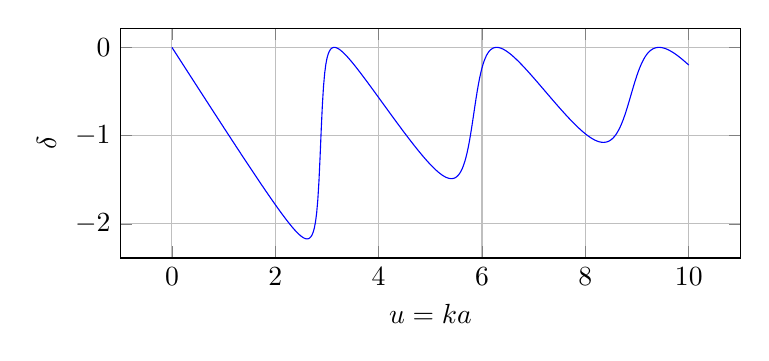
\begin{tikzpicture}
\begin{axis}[width=0.78\textwidth,height=4.5cm,xlabel={$u=ka$},ylabel={$\delta$},grid=major,legend style={font=\small},]
\addplot+[mark=none] coordinates{(1e-05,-9.0909091e-06) (0.0222322,-0.020211063) (0.0444544,-0.040412871) (0.0666766,-0.060614348) (0.0888988,-0.08081533) (0.111121,-0.10101565) (0.1333432,-0.12121514) (0.1555654,-0.14141364) (0.1777876,-0.16161097) (0.2000098,-0.18180697) (0.222232,-0.20200147) (0.2444542,-0.22219429) (0.2666764,-0.24238526) (0.2888986,-0.26257421) (0.3111208,-0.28276095) (0.333343,-0.3029453) (0.3555652,-0.3231271) (0.3777874,-0.34330614) (0.4000096,-0.36348224) (0.4222318,-0.38365521) (0.444454,-0.40382485) (0.4666762,-0.42399098) (0.4888984,-0.44415338) (0.5111206,-0.46431185) (0.5333428,-0.48446619) (0.555565,-0.50461617) (0.5777872,-0.52476158) (0.6000094,-0.54490219) (0.6222316,-0.56503777) (0.6444538,-0.5851681) (0.666676,-0.60529292) (0.6888982,-0.62541199) (0.7111204,-0.64552505) (0.7333426,-0.66563184) (0.7555648,-0.68573209) (0.777787,-0.70582553) (0.8000092,-0.72591186) (0.8222314,-0.74599079) (0.8444536,-0.76606201) (0.8666758,-0.78612521) (0.888898,-0.80618006) (0.9111202,-0.82622622) (0.9333424,-0.84626334) (0.9555646,-0.86629105) (0.9777868,-0.88630898) (1.000009,-0.90631673) (1.0222312,-0.9263139) (1.0444534,-0.94630005) (1.0666756,-0.96627476) (1.0888978,-0.98623755) (1.11112,-1.0061879) (1.1333422,-1.0261254) (1.1555644,-1.0460495) (1.1777866,-1.0659596) (1.2000088,-1.0858552) (1.222231,-1.1057356) (1.2444532,-1.1256002) (1.2666754,-1.1454484) (1.2888976,-1.1652795) (1.3111198,-1.1850926) (1.333342,-1.2048872) (1.3555642,-1.2246622) (1.3777864,-1.244417) (1.4000086,-1.2641505) (1.4222308,-1.2838619) (1.444453,-1.3035501) (1.4666752,-1.323214) (1.4888974,-1.3428526) (1.5111196,-1.3624645) (1.5333418,-1.3820486) (1.555564,-1.4016035) (1.5777862,-1.4211277) (1.6000084,-1.4406196) (1.6222306,-1.4600777) (1.6444528,-1.4795001) (1.666675,-1.498885) (1.6888972,-1.5182304) (1.7111194,-1.537534) (1.7333416,-1.5567936) (1.7555638,-1.5760067) (1.777786,-1.5951704) (1.8000082,-1.614282) (1.8222304,-1.6333382) (1.8444526,-1.6523356) (1.8666748,-1.6712705) (1.888897,-1.6901388) (1.9111192,-1.7089362) (1.9333414,-1.7276578) (1.9555636,-1.7462983) (1.9777858,-1.764852) (2.000008,-1.7833126) (2.0222302,-1.8016729) (2.0444524,-1.8199254) (2.0666746,-1.8380614) (2.0888968,-1.8560714) (2.111119,-1.8739449) (2.1333412,-1.8916701) (2.1555634,-1.9092337) (2.1777856,-1.9266208) (2.2000078,-1.9438146) (2.22223,-1.9607962) (2.2444522,-1.9775438) (2.2666744,-1.9940327) (2.2888966,-2.0102346) (2.3111188,-2.0261168) (2.333341,-2.0416413) (2.3555632,-2.056764) (2.3777854,-2.071433) (2.4000076,-2.0855872) (2.4222298,-2.0991538) (2.444452,-2.1120459) (2.4666742,-2.1241582) (2.4888964,-2.1353626) (2.5111186,-2.1455013) (2.5333408,-2.1543781) (2.555563,-2.1617461) (2.5777852,-2.1672898) (2.6000074,-2.1706013) (2.6222296,-2.1711435) (2.6444518,-2.1681967) (2.666674,-2.1607769) (2.6888962,-2.1475082) (2.7111184,-2.1264197) (2.7333406,-2.0946137) (2.7555628,-2.047722) (2.777785,-1.9790307) (2.8000072,-1.8782261) (2.8222294,-1.730364) (2.8444516,-1.5184891) (2.8666738,-1.2389701) (2.888896,-0.92798322) (2.9111182,-0.64952821) (2.9333404,-0.43892661) (2.9555626,-0.29204707) (2.9777848,-0.19188816) (3.000007,-0.12358984) (3.0222292,-0.076917882) (3.0444514,-0.045212803) (3.0666736,-0.024140512) (3.0888958,-0.010824761) (3.111118,-0.0033080128) (3.1333402,-0.00022322345) (3.1555624,-0.00059219055) (3.1777846,-0.0036991682) (3.2000068,-0.0090097881) (3.222229,-0.016117799) (3.2444512,-0.024709277) (3.2666734,-0.034538057) (3.2888956,-0.045408536) (3.3111178,-0.057163406) (3.33334,-0.069674774) (3.3555622,-0.082837618) (3.3777844,-0.096564903) (3.4000066,-0.1107839) (3.4222288,-0.12543334) (3.444451,-0.14046127) (3.4666732,-0.1558233) (3.4888954,-0.17148129) (3.5111176,-0.18740227) (3.5333398,-0.20355757) (3.555562,-0.21992216) (3.5777842,-0.23647401) (3.6000064,-0.25319372) (3.6222286,-0.27006407) (3.6444508,-0.28706972) (3.666673,-0.30419698) (3.6888952,-0.32143351) (3.7111174,-0.33876821) (3.7333396,-0.35619102) (3.7555618,-0.3736928) (3.777784,-0.3912652) (3.8000062,-0.40890056) (3.8222284,-0.42659185) (3.8444506,-0.44433257) (3.8666728,-0.46211668) (3.888895,-0.47993857) (3.9111172,-0.49779298) (3.9333394,-0.51567499) (3.9555616,-0.53357993) (3.9777838,-0.55150341) (4.000006,-0.56944123) (4.0222282,-0.58738939) (4.0444504,-0.60534403) (4.0666726,-0.62330146) (4.0888948,-0.64125808) (4.111117,-0.6592104) (4.1333392,-0.677155) (4.1555614,-0.69508852) (4.1777836,-0.71300765) (4.2000058,-0.73090911) (4.222228,-0.74878964) (4.2444502,-0.76664597) (4.2666724,-0.78447481) (4.2888946,-0.80227286) (4.3111168,-0.82003678) (4.333339,-0.83776315) (4.3555612,-0.8554485) (4.3777834,-0.87308929) (4.4000056,-0.89068184) (4.4222278,-0.9082224) (4.44445,-0.92570707) (4.4666722,-0.9431318) (4.4888944,-0.96049239) (4.5111166,-0.97778443) (4.5333388,-0.99500334) (4.555561,-1.0121443) (4.5777832,-1.0292022) (4.6000054,-1.0461718) (4.6222276,-1.0630473) (4.6444498,-1.0798228) (4.666672,-1.096492) (4.6888942,-1.113048) (4.7111164,-1.1294838) (4.7333386,-1.1457915) (4.7555608,-1.161963) (4.777783,-1.1779894) (4.8000052,-1.1938613) (4.8222274,-1.2095684) (4.8444496,-1.2250998) (4.8666718,-1.2404436) (4.888894,-1.2555868) (4.9111162,-1.2705156) (4.9333384,-1.2852147) (4.9555606,-1.2996676) (4.9777828,-1.3138562) (5.000005,-1.3277608) (5.0222272,-1.3413597) (5.0444494,-1.3546293) (5.0666716,-1.3675432) (5.0888938,-1.3800727) (5.111116,-1.3921858) (5.1333382,-1.4038471) (5.1555604,-1.4150172) (5.1777826,-1.4256523) (5.2000048,-1.4357034) (5.222227,-1.4451157) (5.2444492,-1.4538275) (5.2666714,-1.4617694) (5.2888936,-1.4688632) (5.3111158,-1.4750201) (5.333338,-1.4801394) (5.3555602,-1.4841064) (5.3777824,-1.4867901) (5.4000046,-1.4880408) (5.4222268,-1.4876866) (5.444449,-1.48553) (5.4666712,-1.4813438) (5.4888934,-1.4748663) (5.5111156,-1.4657965) (5.5333378,-1.4537885) (5.55556,-1.4384464) (5.5777822,-1.4193203) (5.6000044,-1.3959048) (5.6222266,-1.3676413) (5.6444488,-1.3339297) (5.666671,-1.2941517) (5.6888932,-1.2477142) (5.7111154,-1.194119) (5.7333376,-1.1330623) (5.7555598,-1.0645627) (5.777782,-0.98909971) (5.8000042,-0.90772469) (5.8222264,-0.82209097) (5.8444486,-0.73435634) (5.8666708,-0.64694949) (5.888893,-0.5622539) (5.9111152,-0.48230606) (5.9333374,-0.4085967) (5.9555596,-0.34201163) (5.9777818,-0.28288985) (6.000004,-0.23114706) (6.0222262,-0.18641386) (6.0444484,-0.148157) (6.0666706,-0.11577071) (6.0888928,-0.088638239) (6.111115,-0.066168994) (6.1333372,-0.047818348) (6.1555594,-0.033095921) (6.1777816,-0.021566928) (6.2000038,-0.012849615) (6.222226,-0.006610774) (6.2444482,-0.0025605102) (6.2666704,-0.00044696394) (6.2888926,-5.1328429e-05) (6.3111148,-0.0011833416) (6.333337,-0.0036773017) (6.3555592,-0.0073886018) (6.3777814,-0.012190744) (6.4000036,-0.017972782) (6.4222258,-0.024637147) (6.444448,-0.032097784) (6.4666702,-0.040278579) (6.4888924,-0.049112016) (6.5111146,-0.058538025) (6.5333368,-0.068503015) (6.555559,-0.078959033) (6.5777812,-0.089863049) (6.6000034,-0.10117635) (6.6222256,-0.11286399) (6.6444478,-0.12489437) (6.66667,-0.13723882) (6.6888922,-0.14987123) (6.7111144,-0.16276784) (6.7333366,-0.17590687) (6.7555588,-0.18926837) (6.777781,-0.202834) (6.8000032,-0.21658686) (6.8222254,-0.23051131) (6.8444476,-0.24459287) (6.8666698,-0.25881808) (6.888892,-0.27317439) (6.9111142,-0.28765008) (6.9333364,-0.30223417) (6.9555586,-0.31691632) (6.9777808,-0.3316868) (7.000003,-0.3465364) (7.0222252,-0.36145638) (7.0444474,-0.37643842) (7.0666696,-0.3914746) (7.0888918,-0.40655729) (7.111114,-0.42167919) (7.1333362,-0.43683325) (7.1555584,-0.45201261) (7.1777806,-0.46721066) (7.2000028,-0.48242091) (7.222225,-0.49763701) (7.2444472,-0.51285274) (7.2666694,-0.52806195) (7.2888916,-0.54325855) (7.3111138,-0.55843648) (7.333336,-0.57358971) (7.3555582,-0.58871219) (7.3777804,-0.60379784) (7.4000026,-0.61884053) (7.4222248,-0.63383405) (7.444447,-0.64877208) (7.4666692,-0.6636482) (7.4888914,-0.67845583) (7.5111136,-0.69318823) (7.5333358,-0.70783844) (7.555558,-0.72239931) (7.5777802,-0.73686342) (7.6000024,-0.75122306) (7.6222246,-0.76547022) (7.6444468,-0.77959654) (7.666669,-0.79359328) (7.6888912,-0.80745128) (7.7111134,-0.8211609) (7.7333356,-0.83471202) (7.7555578,-0.84809394) (7.77778,-0.86129536) (7.8000022,-0.8743043) (7.8222244,-0.88710808) (7.8444466,-0.89969318) (7.8666688,-0.91204524) (7.888891,-0.92414893) (7.9111132,-0.93598789) (7.9333354,-0.9475446) (7.9555576,-0.9588003) (7.9777798,-0.96973486) (8.000002,-0.98032666) (8.0222242,-0.99055242) (8.0444464,-1.0003871) (8.0666686,-1.0098036) (8.0888908,-1.0187729) (8.111113,-1.0272632) (8.1333352,-1.0352405) (8.1555574,-1.0426678) (8.1777796,-1.049505) (8.2000018,-1.0557086) (8.222224,-1.0612313) (8.2444462,-1.0660218) (8.2666684,-1.0700245) (8.2888906,-1.0731789) (8.3111128,-1.0754191) (8.333335,-1.076674) (8.3555572,-1.0768662) (8.3777794,-1.0759121) (8.4000016,-1.0737215) (8.4222238,-1.0701971) (8.444446,-1.0652348) (8.4666682,-1.0587237) (8.4888904,-1.0505462) (8.5111126,-1.0405792) (8.5333348,-1.0286949) (8.555557,-1.0147632) (8.5777792,-0.99865406) (8.6000014,-0.9802417) (8.6222236,-0.95940922) (8.6444458,-0.93605516) (8.666668,-0.91010122) (8.6888902,-0.8815014) (8.7111124,-0.8502521) (8.7333346,-0.81640271) (8.7555568,-0.78006569) (8.777779,-0.74142473) (8.8000012,-0.70073966) (8.8222234,-0.65834643) (8.8444456,-0.61465099) (8.8666678,-0.57011665) (8.88889,-0.52524537) (8.9111122,-0.48055475) (8.9333344,-0.43655314) (8.9555566,-0.39371581) (8.9777788,-0.35246501) (9.000001,-0.31315562) (9.0222232,-0.27606734) (9.0444454,-0.24140321) (9.0666676,-0.20929337) (9.0888898,-0.17980254) (9.111112,-0.15293974) (9.1333342,-0.12866884) (9.1555564,-0.10691886) (9.1777786,-0.087593429) (9.2000008,-0.070578879) (9.222223,-0.055750989) (9.2444452,-0.042980314) (9.2666674,-0.032136275) (9.2888896,-0.023090172) (9.3111118,-0.015717317) (9.333334,-0.009898457) (9.3555562,-0.005520661) (9.3777784,-0.0024777847) (9.4000006,-0.00067064016) (9.4222228,-6.9480267e-06) (9.444445,-0.00040114091) (9.4666672,-0.0017740699) (9.4888894,-0.0040526512) (9.5111116,-0.0071694813) (9.5333338,-0.01106244) (9.555556,-0.015674295) (9.5777782,-0.020952319) (9.6000004,-0.026847921) (9.6222226,-0.033316303) (9.6444448,-0.040316133) (9.666667,-0.047809251) (9.6888892,-0.055760385) (9.7111114,-0.064136903) (9.7333336,-0.072908577) (9.7555558,-0.082047371) (9.777778,-0.091527245) (9.8000002,-0.10132398) (9.8222224,-0.11141501) (9.8444446,-0.1217793) (9.8666668,-0.13239717) (9.888889,-0.1432502) (9.9111112,-0.15432112) (9.9333334,-0.16559372) (9.9555556,-0.17705271) (9.9777778,-0.18868369) (10,-0.20047304)};
\end{axis}\end{tikzpicture}\end{center}

\begin{center}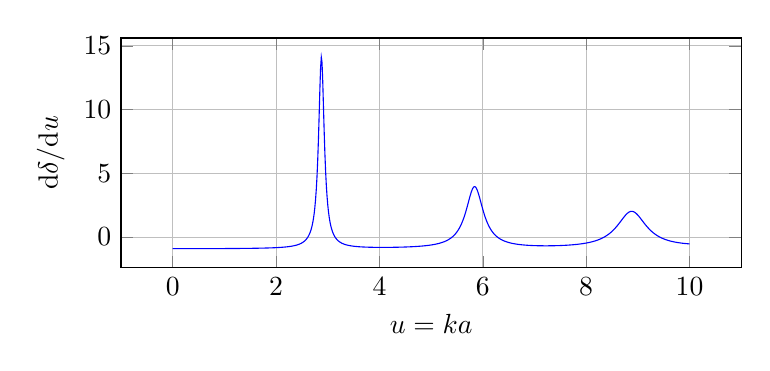
\begin{tikzpicture}
\begin{axis}[width=0.78\textwidth,height=4.5cm,xlabel={$u=ka$},ylabel={$\mathrm d\delta/\mathrm du$},grid=major,legend style={font=\small},]
\addplot+[mark=none] coordinates{(1e-05,-0.90909091) (0.013898875,-0.90908946) (0.02778775,-0.90908511) (0.041676625,-0.90907785) (0.0555655,-0.9090677) (0.069454375,-0.90905464) (0.08334325,-0.90903866) (0.097232125,-0.90901977) (0.111121,-0.90899795) (0.12500987,-0.9089732) (0.13889875,-0.9089455) (0.15278763,-0.90891485) (0.1666765,-0.90888123) (0.18056538,-0.90884464) (0.19445425,-0.90880505) (0.20834313,-0.90876246) (0.222232,-0.90871684) (0.23612088,-0.90866818) (0.25000975,-0.90861645) (0.26389862,-0.90856165) (0.2777875,-0.90850374) (0.29167637,-0.90844271) (0.30556525,-0.90837853) (0.31945413,-0.90831118) (0.333343,-0.90824062) (0.34723188,-0.90816684) (0.36112075,-0.9080898) (0.37500963,-0.90800946) (0.3888985,-0.90792581) (0.40278738,-0.9078388) (0.41667625,-0.90774839) (0.43056512,-0.90765456) (0.444454,-0.90755726) (0.45834288,-0.90745646) (0.47223175,-0.9073521) (0.48612063,-0.90724415) (0.5000095,-0.90713256) (0.51389837,-0.90701728) (0.52778725,-0.90689827) (0.54167612,-0.90677546) (0.555565,-0.90664882) (0.56945387,-0.90651828) (0.58334275,-0.90638379) (0.59723162,-0.90624528) (0.6111205,-0.9061027) (0.62500937,-0.90595598) (0.63889825,-0.90580505) (0.65278712,-0.90564985) (0.666676,-0.9054903) (0.68056487,-0.90532632) (0.69445375,-0.90515785) (0.70834263,-0.9049848) (0.7222315,-0.90480708) (0.73612037,-0.90462462) (0.75000925,-0.90443732) (0.76389812,-0.90424509) (0.777787,-0.90404783) (0.79167587,-0.90384545) (0.80556475,-0.90363784) (0.81945362,-0.9034249) (0.8333425,-0.90320651) (0.84723138,-0.90298256) (0.86112025,-0.90275293) (0.87500912,-0.9025175) (0.888898,-0.90227614) (0.90278687,-0.90202871) (0.91667575,-0.90177509) (0.93056462,-0.90151512) (0.9444535,-0.90124866) (0.95834237,-0.90097555) (0.97223125,-0.90069564) (0.98612013,-0.90040875) (1.000009,-0.90011473) (1.0138979,-0.89981338) (1.0277867,-0.89950453) (1.0416756,-0.89918798) (1.0555645,-0.89886352) (1.0694534,-0.89853096) (1.0833423,-0.89819008) (1.0972311,-0.89784064) (1.11112,-0.89748243) (1.1250089,-0.89711518) (1.1388978,-0.89673866) (1.1527866,-0.89635259) (1.1666755,-0.89595671) (1.1805644,-0.89555072) (1.1944533,-0.89513433) (1.2083421,-0.89470723) (1.222231,-0.8942691) (1.2361199,-0.8938196) (1.2500088,-0.89335837) (1.2638976,-0.89288506) (1.2777865,-0.89239927) (1.2916754,-0.89190061) (1.3055642,-0.89138867) (1.3194531,-0.890863) (1.333342,-0.89032316) (1.3472309,-0.88976866) (1.3611198,-0.889199) (1.3750086,-0.88861368) (1.3888975,-0.88801213) (1.4027864,-0.8873938) (1.4166753,-0.88675808) (1.4305641,-0.88610435) (1.444453,-0.88543195) (1.4583419,-0.88474018) (1.4722308,-0.88402834) (1.4861196,-0.88329566) (1.5000085,-0.88254133) (1.5138974,-0.88176454) (1.5277863,-0.88096438) (1.5416751,-0.88013995) (1.555564,-0.87929026) (1.5694529,-0.87841428) (1.5833417,-0.87751094) (1.5972306,-0.8765791) (1.6111195,-0.87561755) (1.6250084,-0.87462503) (1.6388973,-0.87360019) (1.6527861,-0.87254163) (1.666675,-0.87144784) (1.6805639,-0.87031724) (1.6944528,-0.86914817) (1.7083416,-0.86793883) (1.7222305,-0.86668737) (1.7361194,-0.86539177) (1.7500083,-0.86404993) (1.7638971,-0.86265959) (1.777786,-0.86121837) (1.7916749,-0.85972373) (1.8055638,-0.85817295) (1.8194526,-0.85656316) (1.8333415,-0.85489129) (1.8472304,-0.85315405) (1.8611193,-0.85134793) (1.8750081,-0.84946921) (1.888897,-0.84751386) (1.9027859,-0.8454776) (1.9166748,-0.84335582) (1.9305636,-0.8411436) (1.9444525,-0.83883564) (1.9583414,-0.83642622) (1.9722303,-0.83390922) (1.9861191,-0.83127803) (2.000008,-0.82852551) (2.0138969,-0.82564396) (2.0277858,-0.82262506) (2.0416746,-0.8194598) (2.0555635,-0.81613839) (2.0694524,-0.81265023) (2.0833413,-0.80898379) (2.0972301,-0.80512653) (2.111119,-0.80106476) (2.1250079,-0.79678356) (2.1388968,-0.7922666) (2.1527856,-0.787496) (2.1666745,-0.78245216) (2.1805634,-0.77711354) (2.1944522,-0.77145641) (2.2083411,-0.76545464) (2.22223,-0.75907931) (2.2361189,-0.75229845) (2.2500077,-0.74507657) (2.2638966,-0.7373742) (2.2777855,-0.7291474) (2.2916744,-0.72034705) (2.3055633,-0.71091817) (2.3194521,-0.70079905) (2.333341,-0.68992023) (2.3472299,-0.67820333) (2.3611188,-0.66555962) (2.3750076,-0.65188835) (2.3888965,-0.63707477) (2.4027854,-0.62098776) (2.4166743,-0.60347692) (2.4305631,-0.58436913) (2.444452,-0.56346434) (2.4583409,-0.54053041) (2.4722297,-0.51529679) (2.4861186,-0.48744676) (2.5000075,-0.4566077) (2.5138964,-0.42233903) (2.5277852,-0.38411694) (2.5416741,-0.34131514) (2.555563,-0.29318018) (2.5694519,-0.23879983) (2.5833408,-0.17706196) (2.5972296,-0.10660095) (2.6111185,-0.025726842) (2.6250074,0.067668698) (2.6388963,0.17623873) (2.6527851,0.30335206) (2.666674,0.45332671) (2.6805629,0.63175131) (2.6944518,0.84592978) (2.7083406,1.1054987) (2.7222295,1.4232819) (2.7361184,1.8164571) (2.7500072,2.3080961) (2.7638961,2.9290362) (2.777785,3.7196959) (2.7916739,4.7304623) (2.8055627,6.0168401) (2.8194516,7.6204633) (2.8333405,9.5200833) (2.8472294,11.540588) (2.8611183,13.263958) (2.8750071,14.109314) (2.888896,13.708893) (2.9027849,12.24409) (2.9166738,10.271873) (2.9305626,8.2959338) (2.9444515,6.5749965) (2.9583404,5.1747203) (2.9722293,4.0688443) (2.9861181,3.2035947) (3.000007,2.5256365) (3.0138959,1.9907483) (3.0277847,1.5647282) (3.0416736,1.2218599) (3.0555625,0.94298406) (3.0694514,0.71382064) (3.0833403,0.52366804) (3.0972291,0.36444208) (3.111118,0.22997921) (3.1250069,0.11553437) (3.1388958,0.017418793) (3.1527846,-0.067262541) (3.1666735,-0.14080268) (3.1805624,-0.20503382) (3.1944513,-0.26143219) (3.2083401,-0.31119652) (3.222229,-0.35530753) (3.2361179,-0.39457316) (3.2500068,-0.42966342) (3.2638956,-0.4611374) (3.2777845,-0.48946439) (3.2916734,-0.51504043) (3.3055622,-0.53820154) (3.3194511,-0.5592342) (3.33334,-0.57838381) (3.3472289,-0.59586147) (3.3611178,-0.61184958) (3.3750066,-0.62650633) (3.3888955,-0.63996945) (3.4027844,-0.65235928) (3.4166733,-0.66378131) (3.4305621,-0.67432833) (3.444451,-0.68408219) (3.4583399,-0.69311531) (3.4722288,-0.70149196) (3.4861176,-0.7092693) (3.5000065,-0.71649832) (3.5138954,-0.7232246) (3.5277843,-0.72948898) (3.5416731,-0.73532814) (3.555562,-0.74077511) (3.5694509,-0.74585963) (3.5833397,-0.75060862) (3.5972286,-0.75504642) (3.6111175,-0.75919509) (3.6250064,-0.76307468) (3.6388953,-0.76670344) (3.6527841,-0.77009797) (3.666673,-0.77327343) (3.6805619,-0.77624366) (3.6944508,-0.77902134) (3.7083396,-0.78161805) (3.7222285,-0.78404443) (3.7361174,-0.78631024) (3.7500063,-0.78842444) (3.7638951,-0.79039527) (3.777784,-0.79223032) (3.7916729,-0.79393657) (3.8055618,-0.79552044) (3.8194506,-0.79698788) (3.8333395,-0.79834435) (3.8472284,-0.79959489) (3.8611172,-0.80074415) (3.8750061,-0.80179644) (3.888895,-0.80275571) (3.9027839,-0.80362562) (3.9166728,-0.80440954) (3.9305616,-0.80511056) (3.9444505,-0.80573156) (3.9583394,-0.80627515) (3.9722283,-0.80674374) (3.9861171,-0.80713956) (4.000006,-0.80746463) (4.0138949,-0.80772078) (4.0277837,-0.80790971) (4.0416726,-0.80803294) (4.0555615,-0.80809183) (4.0694504,-0.80808762) (4.0833392,-0.80802141) (4.0972281,-0.80789417) (4.111117,-0.80770673) (4.1250059,-0.80745983) (4.1388947,-0.80715408) (4.1527836,-0.80678998) (4.1666725,-0.80636793) (4.1805614,-0.80588822) (4.1944503,-0.80535104) (4.2083391,-0.80475648) (4.222228,-0.80410453) (4.2361169,-0.8033951) (4.2500057,-0.80262799) (4.2638946,-0.8018029) (4.2777835,-0.80091945) (4.2916724,-0.79997715) (4.3055612,-0.79897543) (4.3194501,-0.79791362) (4.333339,-0.79679095) (4.3472279,-0.79560656) (4.3611167,-0.79435947) (4.3750056,-0.79304862) (4.3888945,-0.79167284) (4.4027834,-0.79023085) (4.4166722,-0.78872126) (4.4305611,-0.78714256) (4.44445,-0.78549315) (4.4583389,-0.78377126) (4.4722278,-0.78197504) (4.4861166,-0.78010249) (4.5000055,-0.77815146) (4.5138944,-0.77611968) (4.5277832,-0.77400471) (4.5416721,-0.77180397) (4.555561,-0.76951468) (4.5694499,-0.76713394) (4.5833387,-0.76465861) (4.5972276,-0.76208539) (4.6111165,-0.75941078) (4.6250054,-0.75663102) (4.6388942,-0.75374218) (4.6527831,-0.75074004) (4.666672,-0.74762013) (4.6805609,-0.74437773) (4.6944497,-0.7410078) (4.7083386,-0.73750501) (4.7222275,-0.73386367) (4.7361164,-0.73007777) (4.7500053,-0.72614089) (4.7638941,-0.72204624) (4.777783,-0.71778656) (4.7916719,-0.71335416) (4.8055607,-0.70874082) (4.8194496,-0.70393783) (4.8333385,-0.69893587) (4.8472274,-0.69372501) (4.8611162,-0.68829468) (4.8750051,-0.68263358) (4.888894,-0.67672963) (4.9027829,-0.67056996) (4.9166717,-0.66414076) (4.9305606,-0.65742729) (4.9444495,-0.65041372) (4.9583384,-0.64308313) (4.9722272,-0.63541735) (4.9861161,-0.62739686) (5.000005,-0.61900073) (5.0138939,-0.61020642) (5.0277828,-0.6009897) (5.0416716,-0.59132445) (5.0555605,-0.58118253) (5.0694494,-0.57053359) (5.0833382,-0.55934483) (5.0972271,-0.5475808) (5.111116,-0.53520317) (5.1250049,-0.52217039) (5.1388937,-0.50843745) (5.1527826,-0.49395549) (5.1666715,-0.47867146) (5.1805604,-0.46252764) (5.1944492,-0.44546126) (5.2083381,-0.4274039) (5.222227,-0.40828094) (5.2361159,-0.38801096) (5.2500047,-0.36650494) (5.2638936,-0.34366556) (5.2777825,-0.31938624) (5.2916714,-0.29355023) (5.3055603,-0.26602946) (5.3194491,-0.23668339) (5.333338,-0.20535766) (5.3472269,-0.17188263) (5.3611157,-0.13607176) (5.3750046,-0.097719919) (5.3888935,-0.056601408) (5.4027824,-0.012467984) (5.4166712,0.034953323) (5.4305601,0.085962468) (5.444449,0.14088868) (5.4583379,0.20009274) (5.4722267,0.26396907) (5.4861156,0.33294753) (5.5000045,0.40749464) (5.5138934,0.48811383) (5.5277822,0.57534437) (5.5416711,0.66975824) (5.55556,0.77195404) (5.5694489,0.88254696) (5.5833377,1.0021532) (5.5972266,1.1313671) (5.6111155,1.2707287) (5.6250044,1.4206796) (5.6388932,1.5815031) (5.6527821,1.7532484) (5.666671,1.935634) (5.6805599,2.1279332) (5.6944487,2.3288423) (5.7083376,2.5363413) (5.7222265,2.7475621) (5.7361154,2.9586868) (5.7500042,3.1649109) (5.7638931,3.3605078) (5.777782,3.539033) (5.7916709,3.6936881) (5.8055597,3.8178394) (5.8194486,3.9056412) (5.8333375,3.9526742) (5.8472264,3.9564784) (5.8611152,3.9168691) (5.8750041,3.8359607) (5.888893,3.7178942) (5.9027819,3.5683312) (5.9166707,3.393824) (5.9305596,3.2011831) (5.9444485,2.9969377) (5.9583374,2.7869454) (5.9722262,2.5761642) (5.9861151,2.3685675) (6.000004,2.1671684) (6.0138929,1.9741127) (6.0277817,1.7908081) (6.0416706,1.6180637) (6.0555595,1.4562231) (6.0694484,1.3052829) (6.0833372,1.1649912) (6.0972261,1.0349273) (6.111115,0.91456355) (6.1250039,0.80331186) (6.1388927,0.70055792) (6.1527816,0.60568532) (6.1666705,0.5180922) (6.1805594,0.43720204) (6.1944482,0.36247027) (6.2083371,0.29338785) (6.222226,0.22948256) (6.2361149,0.17031897) (6.2500037,0.11549733) (6.2638926,0.064651845) (6.2777815,0.017448604) (6.2916704,-0.026416648) (6.3055592,-0.067220822) (6.3194481,-0.10521575) (6.333337,-0.14063037) (6.3472259,-0.17367276) (6.3611147,-0.20453209) (6.3750036,-0.23338038) (6.3888925,-0.2603741) (6.4027814,-0.2856557) (6.4166702,-0.30935494) (6.4305591,-0.33159008) (6.444448,-0.35246902) (6.4583369,-0.3720903) (6.4722257,-0.39054395) (6.4861146,-0.40791235) (6.5000035,-0.42427091) (6.5138924,-0.43968877) (6.5277812,-0.45422932) (6.5416701,-0.46795081) (6.555559,-0.48090675) (6.5694479,-0.49314638) (6.5833367,-0.50471507) (6.5972256,-0.51565459) (6.6111145,-0.52600353) (6.6250034,-0.53579749) (6.6388922,-0.54506938) (6.6527811,-0.55384965) (6.66667,-0.56216648) (6.6805589,-0.57004599) (6.6944477,-0.57751239) (6.7083366,-0.58458815) (6.7222255,-0.59129414) (6.7361144,-0.59764975) (6.7500032,-0.603673) (6.7638921,-0.60938067) (6.777781,-0.61478837) (6.7916699,-0.61991065) (6.8055587,-0.62476107) (6.8194476,-0.62935225) (6.8333365,-0.63369599) (6.8472254,-0.63780329) (6.8611142,-0.6416844) (6.8750031,-0.64534892) (6.888892,-0.64880578) (6.9027809,-0.65206334) (6.9166697,-0.6551294) (6.9305586,-0.65801124) (6.9444475,-0.66071567) (6.9583364,-0.66324903) (6.9722252,-0.66561725) (6.9861141,-0.66782585) (7.000003,-0.66987997) (7.0138919,-0.67178442) (7.0277807,-0.67354364) (7.0416696,-0.6751618) (7.0555585,-0.67664274) (7.0694474,-0.67799001) (7.0833362,-0.67920693) (7.0972251,-0.68029654) (7.111114,-0.68126162) (7.1250029,-0.68210476) (7.1388917,-0.68282829) (7.1527806,-0.68343435) (7.1666695,-0.68392487) (7.1805584,-0.68430158) (7.1944472,-0.68456602) (7.2083361,-0.68471956) (7.222225,-0.68476336) (7.2361139,-0.68469843) (7.2500027,-0.68452562) (7.2638916,-0.6842456) (7.2777805,-0.68385888) (7.2916694,-0.6833658) (7.3055582,-0.68276656) (7.3194471,-0.6820612) (7.333336,-0.68124961) (7.3472249,-0.68033151) (7.3611137,-0.67930649) (7.3750026,-0.67817396) (7.3888915,-0.6769332) (7.4027804,-0.67558333) (7.4166692,-0.67412331) (7.4305581,-0.67255193) (7.444447,-0.67086784) (7.4583359,-0.66906953) (7.4722247,-0.66715529) (7.4861136,-0.66512328) (7.5000025,-0.66297147) (7.5138914,-0.66069764) (7.5277802,-0.6582994) (7.5416691,-0.65577417) (7.555558,-0.65311916) (7.5694469,-0.65033139) (7.5833357,-0.64740766) (7.5972246,-0.64434457) (7.6111135,-0.64113847) (7.6250024,-0.63778548) (7.6388912,-0.63428148) (7.6527801,-0.63062208) (7.666669,-0.62680263) (7.6805579,-0.62281818) (7.6944468,-0.61866351) (7.7083356,-0.61433305) (7.7222245,-0.60982095) (7.7361134,-0.60512098) (7.7500022,-0.60022655) (7.7638911,-0.5951307) (7.77778,-0.58982607) (7.7916689,-0.58430487) (7.8055577,-0.57855885) (7.8194466,-0.5725793) (7.8333355,-0.56635701) (7.8472244,-0.55988224) (7.8611132,-0.55314468) (7.8750021,-0.54613343) (7.888891,-0.53883699) (7.9027799,-0.53124316) (7.9166687,-0.52333904) (7.9305576,-0.51511101) (7.9444465,-0.50654463) (7.9583354,-0.49762463) (7.9722243,-0.48833486) (7.9861131,-0.47865821) (8.000002,-0.46857658) (8.0138909,-0.45807079) (8.0277798,-0.44712056) (8.0416686,-0.43570439) (8.0555575,-0.42379952) (8.0694464,-0.41138186) (8.0833352,-0.39842587) (8.0972241,-0.38490454) (8.111113,-0.37078924) (8.1250019,-0.35604966) (8.1388907,-0.34065371) (8.1527796,-0.32456745) (8.1666685,-0.30775493) (8.1805574,-0.29017814) (8.1944463,-0.27179691) (8.2083351,-0.25256878) (8.222224,-0.23244892) (8.2361129,-0.21139003) (8.2500017,-0.18934227) (8.2638906,-0.16625316) (8.2777795,-0.14206756) (8.2916684,-0.11672757) (8.3055572,-0.090172595) (8.3194461,-0.062339275) (8.333335,-0.033161612) (8.3472239,-0.0025710531) (8.3611128,0.029503328) (8.3750016,0.063134575) (8.3888905,0.098397498) (8.4027794,0.1353682) (8.4166682,0.17412349) (8.4305571,0.21474008) (8.444446,0.25729362) (8.4583349,0.30185754) (8.4722237,0.3485015) (8.4861126,0.39728971) (8.5000015,0.44827874) (8.5138904,0.501515) (8.5277793,0.55703183) (8.5416681,0.61484604) (8.555557,0.67495399) (8.5694459,0.73732711) (8.5833347,0.80190701) (8.5972236,0.86859998) (8.6111125,0.93727116) (8.6250014,1.0077385) (8.6388902,1.0797664) (8.6527791,1.1530599) (8.666668,1.2272591) (8.6805569,1.3019345) (8.6944457,1.3765841) (8.7083346,1.4506325) (8.7222235,1.5234323) (8.7361124,1.5942693) (8.7500013,1.6623714) (8.7638901,1.7269213) (8.777779,1.7870746) (8.7916679,1.8419806) (8.8055567,1.8908081) (8.8194456,1.932773) (8.8333345,1.9671672) (8.8472234,1.9933866) (8.8611122,2.0109574) (8.8750011,2.0195565) (8.88889,2.0190269) (8.9027789,2.0093848) (8.9166678,1.9908191) (8.9305566,1.9636823) (8.9444455,1.9284744) (8.9583344,1.8858208) (8.9722232,1.8364463) (8.9861121,1.7811459) (9.000001,1.7207565) (9.0138899,1.6561297) (9.0277787,1.5881064) (9.0416676,1.5174968) (9.0555565,1.4450632) (9.0694454,1.3715079) (9.0833343,1.2974655) (9.0972231,1.2234977) (9.111112,1.1500931) (9.1250009,1.077668) (9.1388897,1.00657) (9.1527786,0.93708271) (9.1666675,0.86943133) (9.1805564,0.80378881) (9.1944452,0.740282) (9.2083341,0.67899774) (9.222223,0.61998858) (9.2361119,0.5632782) (9.2500007,0.50886624) (9.2638896,0.45673265) (9.2777785,0.40684154) (9.2916674,0.35914451) (9.3055563,0.3135835) (9.3194451,0.2700933) (9.333334,0.22860351) (9.3472229,0.18904034) (9.3611117,0.15132796) (9.3750006,0.11538973) (9.3888895,0.081149035) (9.4027784,0.048530115) (9.4166672,0.017458591) (9.4305561,-0.012138073) (9.444445,-0.040330237) (9.4583339,-0.067185846) (9.4722228,-0.092770271) (9.4861116,-0.1171462) (9.5000005,-0.1403736) (9.5138894,-0.16250968) (9.5277782,-0.18360894) (9.5416671,-0.20372321) (9.555556,-0.22290168) (9.5694449,-0.24119101) (9.5833337,-0.25863543) (9.5972226,-0.2752768) (9.6111115,-0.29115469) (9.6250004,-0.30630657) (9.6388893,-0.32076779) (9.6527781,-0.33457179) (9.666667,-0.34775012) (9.6805559,-0.36033257) (9.6944447,-0.37234728) (9.7083336,-0.38382079) (9.7222225,-0.39477814) (9.7361114,-0.40524297) (9.7500002,-0.41523759) (9.7638891,-0.42478305) (9.777778,-0.4338992) (9.7916669,-0.44260479) (9.8055557,-0.4509175) (9.8194446,-0.45885402) (9.8333335,-0.46643009) (9.8472224,-0.47366058) (9.8611113,-0.48055953) (9.8750001,-0.48714016) (9.888889,-0.49341497) (9.9027779,-0.49939575) (9.9166667,-0.50509363) (9.9305556,-0.51051911) (9.9444445,-0.51568211) (9.9583334,-0.52059196) (9.9722222,-0.52525748) (9.9861111,-0.52968699) (10,-0.53380654)};
\end{axis}\end{tikzpicture}\end{center}

\begin{center}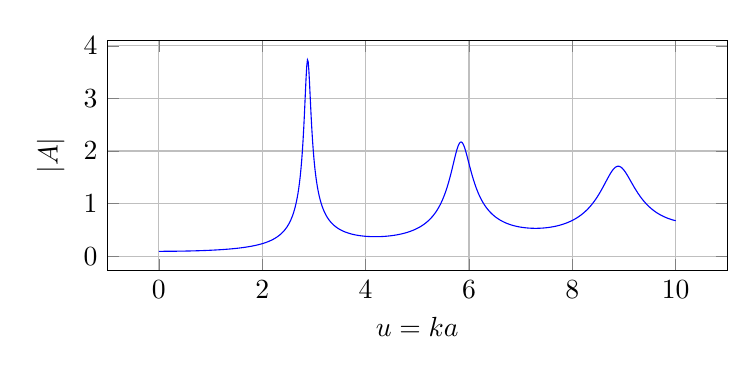
\begin{tikzpicture}
\begin{axis}[width=0.78\textwidth,height=4.5cm,xlabel={$u=ka$},ylabel={$|A|$},grid=major,legend style={font=\small},]
\addplot+[mark=none] coordinates{(1e-05,0.090909091) (0.013898875,0.090912478) (0.02778775,0.090922629) (0.041676625,0.090939548) (0.0555655,0.09096324) (0.069454375,0.090993713) (0.08334325,0.091030977) (0.097232125,0.091075042) (0.111121,0.091125924) (0.12500987,0.091183638) (0.13889875,0.091248203) (0.15278763,0.09131964) (0.1666765,0.09139797) (0.18056538,0.09148322) (0.19445425,0.091575416) (0.20834313,0.091674588) (0.222232,0.091780768) (0.23612088,0.091893991) (0.25000975,0.092014292) (0.26389862,0.092141711) (0.2777875,0.092276288) (0.29167637,0.092418068) (0.30556525,0.092567098) (0.31945413,0.092723424) (0.333343,0.0928871) (0.34723188,0.093058178) (0.36112075,0.093236716) (0.37500963,0.093422771) (0.3888985,0.093616407) (0.40278738,0.093817688) (0.41667625,0.09402668) (0.43056512,0.094243455) (0.444454,0.094468085) (0.45834288,0.094700646) (0.47223175,0.094941219) (0.48612063,0.095189884) (0.5000095,0.095446727) (0.51389837,0.095711837) (0.52778725,0.095985306) (0.54167612,0.096267229) (0.555565,0.096557705) (0.56945387,0.096856837) (0.58334275,0.097164729) (0.59723162,0.097481492) (0.6111205,0.097807239) (0.62500937,0.098142087) (0.63889825,0.098486159) (0.65278712,0.098839578) (0.666676,0.099202475) (0.68056487,0.099574985) (0.69445375,0.099957244) (0.70834263,0.1003494) (0.7222315,0.10075159) (0.73612037,0.10116398) (0.75000925,0.10158672) (0.76389812,0.10201997) (0.777787,0.10246391) (0.79167587,0.1029187) (0.80556475,0.10338452) (0.81945362,0.10386157) (0.8333425,0.10435002) (0.84723138,0.10485008) (0.86112025,0.10536195) (0.87500912,0.10588584) (0.888898,0.10642197) (0.90278687,0.10697056) (0.91667575,0.10753184) (0.93056462,0.10810606) (0.9444535,0.10869344) (0.95834237,0.10929426) (0.97223125,0.10990877) (0.98612013,0.11053725) (1.000009,0.11117997) (1.0138979,0.11183722) (1.0277867,0.1125093) (1.0416756,0.11319652) (1.0555645,0.11389921) (1.0694534,0.11461768) (1.0833423,0.11535228) (1.0972311,0.11610336) (1.11112,0.11687128) (1.1250089,0.11765643) (1.1388978,0.11845919) (1.1527866,0.11927996) (1.1666755,0.12011915) (1.1805644,0.12097721) (1.1944533,0.12185458) (1.2083421,0.12275171) (1.222231,0.12366908) (1.2361199,0.1246072) (1.2500088,0.12556657) (1.2638976,0.12654772) (1.2777865,0.1275512) (1.2916754,0.12857759) (1.3055642,0.12962747) (1.3194531,0.13070146) (1.333342,0.13180019) (1.3472309,0.13292432) (1.3611198,0.13407455) (1.3750086,0.13525157) (1.3888975,0.13645612) (1.4027864,0.13768898) (1.4166753,0.13895094) (1.4305641,0.14024283) (1.444453,0.14156551) (1.4583419,0.14291987) (1.4722308,0.14430684) (1.4861196,0.1457274) (1.5000085,0.14718255) (1.5138974,0.14867335) (1.5277863,0.15020089) (1.5416751,0.1517663) (1.555564,0.15337079) (1.5694529,0.1550156) (1.5833417,0.156702) (1.5972306,0.15843137) (1.6111195,0.16020511) (1.6250084,0.1620247) (1.6388973,0.16389168) (1.6527861,0.16580766) (1.666675,0.16777433) (1.6805639,0.16979345) (1.6944528,0.17186689) (1.7083416,0.17399656) (1.7222305,0.17618451) (1.7361194,0.17843287) (1.7500083,0.18074387) (1.7638971,0.18311986) (1.777786,0.1855633) (1.7916749,0.18807681) (1.8055638,0.19066309) (1.8194526,0.19332502) (1.8333415,0.19606563) (1.8472304,0.1988881) (1.8611193,0.2017958) (1.8750081,0.20479227) (1.888897,0.20788125) (1.9027859,0.21106671) (1.9166748,0.21435283) (1.9305636,0.21774404) (1.9444525,0.22124503) (1.9583414,0.22486079) (1.9722303,0.22859658) (1.9861191,0.23245801) (2.000008,0.23645103) (2.0138969,0.24058199) (2.0277858,0.24485763) (2.0416746,0.24928514) (2.0555635,0.25387219) (2.0694524,0.25862697) (2.0833413,0.26355823) (2.0972301,0.26867537) (2.111119,0.2739884) (2.1250079,0.27950812) (2.1388968,0.28524609) (2.1527856,0.29121474) (2.1666745,0.2974275) (2.1805634,0.30389879) (2.1944522,0.31064421) (2.2083411,0.31768065) (2.22223,0.32502635) (2.2361189,0.33270114) (2.2500077,0.34072654) (2.2638966,0.34912596) (2.2777855,0.35792496) (2.2916744,0.36715142) (2.3055633,0.37683585) (2.3194521,0.38701172) (2.333341,0.39771578) (2.3472299,0.40898853) (2.3611188,0.42087463) (2.3750076,0.43342351) (2.3888965,0.44668998) (2.4027854,0.46073496) (2.4166743,0.47562641) (2.4305631,0.4914403) (2.444452,0.50826181) (2.4583409,0.5261868) (2.4722297,0.54532346) (2.4861186,0.56579435) (2.5000075,0.58773882) (2.5138964,0.61131591) (2.5277852,0.63670788) (2.5416741,0.66412452) (2.555563,0.69380839) (2.5694519,0.72604131) (2.5833408,0.76115231) (2.5972296,0.79952763) (2.6111185,0.84162311) (2.6250074,0.88797986) (2.6388963,0.93924396) (2.6527851,0.99619149) (2.666674,1.0597602) (2.6805629,1.1310895) (2.6944518,1.2115711) (2.7083406,1.3029115) (2.7222295,1.407206) (2.7361184,1.5270219) (2.7500072,1.6654749) (2.7638961,1.8262593) (2.777785,2.0135375) (2.7916739,2.2314736) (2.8055627,2.4829673) (2.8194516,2.7667906) (2.8333405,3.0721146) (2.8472294,3.3706079) (2.8611183,3.611549) (2.8750071,3.7335359) (2.888896,3.6992242) (2.9027849,3.5241332) (2.9166738,3.263311) (2.9305626,2.9738908) (2.9444515,2.6933109) (2.9583404,2.4390407) (2.9722293,2.216043) (2.9861181,2.0232322) (3.000007,1.8572243) (3.0138959,1.7141351) (3.0277847,1.5903231) (3.0416736,1.4826329) (3.0555625,1.3884261) (3.0694514,1.3055312) (3.0833403,1.2321716) (3.0972291,1.1668949) (3.111118,1.1085104) (3.1250069,1.0560378) (3.1388958,1.0086663) (3.1527846,0.96572096) (3.1666735,0.9266371) (3.1805624,0.89093943) (3.1944513,0.85822563) (3.2083401,0.82815332) (3.222229,0.80042961) (3.2361179,0.77480262) (3.2500068,0.75105476) (3.2638956,0.7289972) (3.2777845,0.70846533) (3.2916734,0.68931507) (3.3055622,0.67141983) (3.3194511,0.65466796) (3.33334,0.63896068) (3.3472289,0.62421022) (3.3611178,0.61033845) (3.3750066,0.59727552) (3.3888955,0.58495886) (3.4027844,0.57333225) (3.4166733,0.56234505) (3.4305621,0.55195152) (3.444451,0.54211026) (3.4583399,0.53278371) (3.4722288,0.52393773) (3.4861176,0.51554122) (3.5000065,0.50756577) (3.5138954,0.49998544) (3.5277843,0.49277642) (3.5416731,0.48591691) (3.555562,0.47938683) (3.5694509,0.47316772) (3.5833397,0.46724256) (3.5972286,0.46159564) (3.6111175,0.45621243) (3.6250064,0.45107949) (3.6388953,0.44618436) (3.6527841,0.44151549) (3.666673,0.43706214) (3.6805619,0.43281434) (3.6944508,0.42876281) (3.7083396,0.4248989) (3.7222285,0.42121455) (3.7361174,0.41770226) (3.7500063,0.41435499) (3.7638951,0.41116621) (3.777784,0.40812978) (3.7916729,0.40523997) (3.8055618,0.40249144) (3.8194506,0.39987916) (3.8333395,0.39739845) (3.8472284,0.3950449) (3.8611172,0.3928144) (3.8750061,0.39070309) (3.888895,0.38870737) (3.9027839,0.38682384) (3.9166728,0.38504935) (3.9305616,0.38338094) (3.9444505,0.38181581) (3.9583394,0.3803514) (3.9722283,0.37898527) (3.9861171,0.37771516) (4.000006,0.37653897) (4.0138949,0.37545474) (4.0277837,0.37446063) (4.0416726,0.37355496) (4.0555615,0.37273616) (4.0694504,0.37200279) (4.0833392,0.37135351) (4.0972281,0.37078711) (4.111117,0.37030246) (4.1250059,0.36989856) (4.1388947,0.36957449) (4.1527836,0.36932944) (4.1666725,0.36916268) (4.1805614,0.36907357) (4.1944503,0.36906158) (4.2083391,0.36912625) (4.222228,0.36926718) (4.2361169,0.36948411) (4.2500057,0.3697768) (4.2638946,0.37014513) (4.2777835,0.37058905) (4.2916724,0.37110858) (4.3055612,0.37170383) (4.3194501,0.37237497) (4.333339,0.37312227) (4.3472279,0.37394607) (4.3611167,0.37484677) (4.3750056,0.37582487) (4.3888945,0.37688095) (4.4027834,0.37801565) (4.4166722,0.3792297) (4.4305611,0.38052393) (4.44445,0.38189923) (4.4583389,0.38335659) (4.4722278,0.38489707) (4.4861166,0.38652183) (4.5000055,0.38823213) (4.5138944,0.39002931) (4.5277832,0.39191481) (4.5416721,0.39389018) (4.555561,0.39595706) (4.5694499,0.39811721) (4.5833387,0.40037247) (4.5972276,0.40272484) (4.6111165,0.4051764) (4.6250054,0.40772939) (4.6388942,0.41038613) (4.6527831,0.41314914) (4.666672,0.41602101) (4.6805609,0.41900454) (4.6944497,0.42210265) (4.7083386,0.42531842) (4.7222275,0.42865512) (4.7361164,0.43211618) (4.7500053,0.43570524) (4.7638941,0.43942611) (4.777783,0.44328282) (4.7916719,0.44727962) (4.8055607,0.45142101) (4.8194496,0.4557117) (4.8333385,0.46015668) (4.8472274,0.46476121) (4.8611162,0.46953084) (4.8750051,0.47447142) (4.888894,0.47958915) (4.9027829,0.48489054) (4.9166717,0.4903825) (4.9305606,0.49607231) (4.9444495,0.50196768) (4.9583384,0.50807675) (4.9722272,0.51440814) (4.9861161,0.52097097) (5.000005,0.5277749) (5.0138939,0.53483016) (5.0277828,0.54214759) (5.0416716,0.5497387) (5.0555605,0.55761568) (5.0694494,0.56579148) (5.0833382,0.57427985) (5.0972271,0.58309542) (5.111116,0.59225371) (5.1250049,0.60177125) (5.1388937,0.61166563) (5.1527826,0.62195559) (5.1666715,0.63266109) (5.1805604,0.64380341) (5.1944492,0.65540523) (5.2083381,0.66749078) (5.222227,0.6800859) (5.2361159,0.6932182) (5.2500047,0.70691719) (5.2638936,0.72121438) (5.2777825,0.73614348) (5.2916714,0.75174051) (5.3055603,0.768044) (5.3194491,0.78509512) (5.333338,0.80293791) (5.3472269,0.82161939) (5.3611157,0.84118979) (5.3750046,0.86170271) (5.3888935,0.88321523) (5.4027824,0.9057881) (5.4166712,0.92948581) (5.4305601,0.95437663) (5.444449,0.98053259) (5.4583379,1.0080293) (5.4722267,1.0369458) (5.4861156,1.0673639) (5.5000045,1.0993676) (5.5138934,1.133042) (5.5277822,1.1684716) (5.5416711,1.2057387) (5.55556,1.2449201) (5.5694489,1.2860837) (5.5833377,1.3292836) (5.5972266,1.3745538) (5.6111155,1.4219006) (5.6250044,1.4712922) (5.6388932,1.5226477) (5.6527821,1.5758218) (5.666671,1.6305893) (5.6805599,1.6866266) (5.6944487,1.7434926) (5.7083376,1.8006117) (5.7222265,1.8572592) (5.7361154,1.9125546) (5.7500042,1.9654674) (5.7638931,2.0148385) (5.777782,2.0594232) (5.7916709,2.0979554) (5.8055597,2.1292322) (5.8194486,2.1522094) (5.8333375,2.1660969) (5.8472264,2.1704368) (5.8611152,2.1651506) (5.8750041,2.1505463) (5.888893,2.1272822) (5.9027819,2.096298) (5.9166707,2.0587238) (5.9305596,2.0157843) (5.9444485,1.9687118) (5.9583374,1.9186758) (5.9722262,1.8667346) (5.9861151,1.8138076) (6.000004,1.7606646) (6.0138929,1.7079289) (6.0277817,1.6560882) (6.0416706,1.6055107) (6.0555595,1.556463) (6.0694484,1.509127) (6.0833372,1.4636173) (6.0972261,1.4199943) (6.111115,1.3782774) (6.1250039,1.3384546) (6.1388927,1.3004909) (6.1527816,1.2643352) (6.1666705,1.2299246) (6.1805594,1.1971894) (6.1944482,1.1660557) (6.2083371,1.1364474) (6.222226,1.1082887) (6.2361149,1.0815045) (6.2500037,1.0560218) (6.2638926,1.0317703) (6.2777815,1.0086824) (6.2916704,0.98669389) (6.3055592,0.96574377) (6.3194481,0.94577437) (6.333337,0.92673131) (6.3472259,0.90856341) (6.3611147,0.89122258) (6.3750036,0.87466369) (6.3888925,0.85884441) (6.4027814,0.84372507) (6.4166702,0.82926853) (6.4305591,0.81543997) (6.444448,0.80220682) (6.4583369,0.78953857) (6.4722257,0.77740662) (6.4861146,0.76578422) (6.5000035,0.75464626) (6.5138924,0.74396926) (6.5277812,0.73373115) (6.5416701,0.72391127) (6.555559,0.71449021) (6.5694479,0.70544976) (6.5833367,0.69677281) (6.5972256,0.6884433) (6.6111145,0.68044611) (6.6250034,0.67276704) (6.6388922,0.66539272) (6.6527811,0.65831057) (6.66667,0.65150873) (6.6805589,0.64497606) (6.6944477,0.63870202) (6.7083366,0.6326767) (6.7222255,0.62689074) (6.7361144,0.62133532) (6.7500032,0.6160021) (6.7638921,0.61088322) (6.777781,0.60597125) (6.7916699,0.60125918) (6.8055587,0.59674037) (6.8194476,0.59240857) (6.8333365,0.58825784) (6.8472254,0.5842826) (6.8611142,0.58047755) (6.8750031,0.5768377) (6.888892,0.57335831) (6.9027809,0.57003493) (6.9166697,0.56686332) (6.9305586,0.5638395) (6.9444475,0.5609597) (6.9583364,0.55822036) (6.9722252,0.55561813) (6.9861141,0.55314984) (7.000003,0.5508125) (7.0138919,0.5486033) (7.0277807,0.5465196) (7.0416696,0.54455891) (7.0555585,0.54271889) (7.0694474,0.54099734) (7.0833362,0.53939223) (7.0972251,0.53790163) (7.111114,0.53652376) (7.1250029,0.53525695) (7.1388917,0.53409966) (7.1527806,0.53305046) (7.1666695,0.53210805) (7.1805584,0.53127122) (7.1944472,0.53053888) (7.2083361,0.52991003) (7.222225,0.52938377) (7.2361139,0.52895932) (7.2500027,0.52863598) (7.2638916,0.52841315) (7.2777805,0.52829031) (7.2916694,0.52826706) (7.3055582,0.52834306) (7.3194471,0.52851807) (7.333336,0.52879194) (7.3472249,0.52916462) (7.3611137,0.52963612) (7.3750026,0.53020656) (7.3888915,0.53087613) (7.4027804,0.53164512) (7.4166692,0.5325139) (7.4305581,0.53348291) (7.444447,0.53455271) (7.4583359,0.53572393) (7.4722247,0.53699728) (7.4861136,0.53837358) (7.5000025,0.53985372) (7.5138914,0.5414387) (7.5277802,0.5431296) (7.5416691,0.54492759) (7.555558,0.54683397) (7.5694469,0.54885009) (7.5833357,0.55097744) (7.5972246,0.5532176) (7.6111135,0.55557225) (7.6250024,0.55804319) (7.6388912,0.56063232) (7.6527801,0.56334165) (7.666669,0.56617334) (7.6805579,0.56912963) (7.6944468,0.57221291) (7.7083356,0.5754257) (7.7222245,0.57877065) (7.7361134,0.58225053) (7.7500022,0.58586829) (7.7638911,0.589627) (7.77778,0.59352989) (7.7916689,0.59758035) (7.8055577,0.60178194) (7.8194466,0.60613839) (7.8333355,0.6106536) (7.8472244,0.61533167) (7.8611132,0.62017688) (7.8750021,0.6251937) (7.888891,0.63038683) (7.9027799,0.63576118) (7.9166687,0.64132187) (7.9305576,0.64707427) (7.9444465,0.65302396) (7.9583354,0.65917682) (7.9722243,0.66553895) (7.9861131,0.67211673) (8.000002,0.67891683) (8.0138909,0.68594619) (8.0277798,0.69321207) (8.0416686,0.70072203) (8.0555575,0.70848395) (8.0694464,0.71650603) (8.0833352,0.72479683) (8.0972241,0.73336524) (8.111113,0.74222051) (8.1250019,0.75137226) (8.1388907,0.76083046) (8.1527796,0.77060548) (8.1666685,0.78070804) (8.1805574,0.79114925) (8.1944463,0.80194059) (8.2083351,0.81309391) (8.222224,0.8246214) (8.2361129,0.83653561) (8.2500017,0.84884939) (8.2638906,0.8615759) (8.2777795,0.87472853) (8.2916684,0.88832088) (8.3055572,0.9023667) (8.3194461,0.91687979) (8.333335,0.93187395) (8.3472239,0.94736284) (8.3611128,0.96335984) (8.3750016,0.97987795) (8.3888905,0.99692953) (8.4027794,1.0145261) (8.4166682,1.0326782) (8.4305571,1.0513948) (8.444446,1.0706834) (8.4583349,1.0905491) (8.4722237,1.1109945) (8.4861126,1.1320192) (8.5000015,1.1536189) (8.5138904,1.1757851) (8.5277793,1.1985039) (8.5416681,1.2217557) (8.555557,1.2455138) (8.5694459,1.2697439) (8.5833347,1.2944025) (8.5972236,1.3194366) (8.6111125,1.3447817) (8.6250014,1.3703615) (8.6388902,1.3960865) (8.6527791,1.4218532) (8.666668,1.4475435) (8.6805569,1.4730243) (8.6944457,1.4981474) (8.7083346,1.5227501) (8.7222235,1.5466559) (8.7361124,1.5696769) (8.7500013,1.5916155) (8.7638901,1.6122679) (8.777779,1.6314283) (8.7916679,1.6488929) (8.8055567,1.664466) (8.8194456,1.6779648) (8.8333345,1.6892255) (8.8472234,1.6981087) (8.8611122,1.704504) (8.8750011,1.7083344) (8.88889,1.7095591) (8.9027789,1.7081749) (8.9166678,1.7042162) (8.9305566,1.6977535) (8.9444455,1.688891) (8.9583344,1.6777619) (8.9722232,1.6645244) (8.9861121,1.6493555) (9.000001,1.6324462) (9.0138899,1.6139952) (9.0277787,1.5942044) (9.0416676,1.5732739) (9.0555565,1.5513984) (9.0694454,1.5287635) (9.0833343,1.5055439) (9.0972231,1.4819012) (9.111112,1.457983) (9.1250009,1.4339223) (9.1388897,1.4098378) (9.1527786,1.3858338) (9.1666675,1.3620011) (9.1805564,1.3384175) (9.1944452,1.3151492) (9.2083341,1.2922516) (9.222223,1.26977) (9.2361119,1.2477412) (9.2500007,1.2261942) (9.2638896,1.205151) (9.2777785,1.1846279) (9.2916674,1.1646359) (9.3055563,1.1451814) (9.3194451,1.1262674) (9.333334,1.1078935) (9.3472229,1.0900566) (9.3611117,1.0727516) (9.3750006,1.0559712) (9.3888895,1.039707) (9.4027784,1.0239494) (9.4166672,1.0086876) (9.4305561,0.99391038) (9.444445,0.97960594) (9.4583339,0.96576212) (9.4722228,0.95236654) (9.4861116,0.93940675) (9.5000005,0.92687027) (9.5138894,0.91474471) (9.5277782,0.90301781) (9.5416671,0.8916775) (9.555556,0.88071192) (9.5694449,0.87010949) (9.5833337,0.85985893) (9.5972226,0.84994922) (9.6111115,0.8403697) (9.6250004,0.83111003) (9.6388893,0.82216018) (9.6527781,0.81351049) (9.666667,0.80515162) (9.6805559,0.79707456) (9.6944447,0.78927063) (9.7083336,0.78173149) (9.7222225,0.77444911) (9.7361114,0.76741577) (9.7500002,0.76062405) (9.7638891,0.75406684) (9.777778,0.74773731) (9.7916669,0.74162891) (9.8055557,0.73573536) (9.8194446,0.73005064) (9.8333335,0.72456899) (9.8472224,0.71928489) (9.8611113,0.71419305) (9.8750001,0.70928843) (9.888889,0.70456618) (9.9027779,0.70002167) (9.9166667,0.6956505) (9.9305556,0.69144842) (9.9444445,0.68741141) (9.9583334,0.68353562) (9.9722222,0.67981737) (9.9861111,0.67625315) (10,0.67283962)};
\end{axis}\end{tikzpicture}\end{center}

内区驻留增强与大正延迟标识共振, 但势全为非负, 没有负能束缚态. $\delta(0)=\delta(\infty)=0$, 满足$N=0$; 局部相移急升不等于新增束缚态.
\end{solution}
\originalsection{第5题：$z$角动量对易子（10分）}
\begin{exercise}
(a,b)求$L_z$与$x,y,z,p_x,p_y,p_z$的对易子. (c,d)证明$L_z$本征态中$x,y,p_x,p_y$均值为0.
\end{exercise}
\begin{solution}
$L_z=xp_y-yp_x$给$[L_z,x]=\ii\hbar y$,$[L_z,y]=-\ii\hbar x$,$[L_z,z]=0$; 类似$[L_z,p_x]=\ii\hbar p_y$,$[L_z,p_y]=-\ii\hbar p_x$,$[L_z,p_z]=0$. 归一化本征态中$\langle[L_z,A]\rangle=0$, 因为左右$L_z$读数相同. 分别代入上述四个非零式就得到四个均值0, 前提是矩存在和共同定义域允许操作. 不是说这些测量没有分散或粒子停在轴线上.
\end{solution}
\originalsection{第6题：球坐标算符（10分）}
\begin{exercise}
(a)求$r,\theta,\phi$对$x,y,z$的九个导数. (b)写$L_x,L_y,L_z$. (c)分别展开平方并相加得到$L^2$.
\end{exercise}
\begin{solution}
在坐标非奇点, 各行分别为$\nabla r,\nabla\theta,\nabla\phi$:
\[
\begin{pmatrix}
\sin\theta\cos\phi&\sin\theta\sin\phi&\cos\theta\\
\cos\theta\cos\phi/r&\cos\theta\sin\phi/r&-\sin\theta/r\\
-\sin\phi/(r\sin\theta)&\cos\phi/(r\sin\theta)&0
\end{pmatrix}.
\]
链式法则给$L_x=\ii\hbar(\sin\phi\,\partial_\theta+\cot\theta\cos\phi\,\partial_\phi)$,$L_y=\ii\hbar(-\cos\phi\,\partial_\theta+\cot\theta\sin\phi\,\partial_\phi)$,$L_z=-\ii\hbar\partial_\phi$. 为展示平方时对系数也要求导, 令$s=\sin\phi,c=\cos\phi,t=\cot\theta$, 写$L_x=\ii\hbar A,L_y=\ii\hbar B$:
\[
\begin{aligned}
A^2&=s^2\partial_{\theta\theta}+2sct\partial_{\theta\phi}+c^2t^2\partial_{\phi\phi}
+tc^2\partial_\theta-sc(\csc^2\theta+t^2)\partial_\phi,\\
B^2&=c^2\partial_{\theta\theta}-2sct\partial_{\theta\phi}+s^2t^2\partial_{\phi\phi}
+ts^2\partial_\theta+sc(\csc^2\theta+t^2)\partial_\phi.
\end{aligned}
\]
$L_x^2=-\hbar^2A^2,L_y^2=-\hbar^2B^2,L_z^2=-\hbar^2\partial_{\phi\phi}$, 相加混合项抵消, 用$1+\cot^2\theta=\csc^2\theta$得到第10章的$L^2$表达. 轴上的坐标奇点需要正则球面函数解释, 不能直接代$r\sin\theta=0$到导数分式.
\end{solution}
